% Template LaTeX file for DAFx-20 papers
%
% To generate the correct references using BibTeX, run
%     latex, bibtex, latex, latex
% modified...
% - from DAFx-00 to DAFx-02 by Florian Keiler, 2002-07-08
% - from DAFx-03 to DAFx-04 by Gianpaolo Evangelista, 2004-02-07 
% - from DAFx-05 to DAFx-06 by Vincent Verfaille, 2006-02-05
% - from DAFx-06 to DAFx-07 by Vincent Verfaille, 2007-01-05
%                          and Sylvain Marchand, 2007-01-31
% - from DAFx-07 to DAFx-08 by Henri Penttinen, 2007-12-12
%                          and Jyri Pakarinen 2008-01-28
% - from DAFx-08 to DAFx-09 by Giorgio Prandi, Fabio Antonacci 2008-10-03
% - from DAFx-09 to DAFx-10 by Hannes Pomberger 2010-02-01
% - from DAFx-10 to DAFx-12 by Jez Wells 2011
% - from DAFx-12 to DAFx-14 by Sascha Disch 2013
% - from DAFx-15 to DAFx-16 by Pavel Rajmic 2015
% - from DAFx-16 to DAFx-17 by Brian Hamilton 2016
% - from DAFx-17 to DAFx-18 by Annibal Ferreira and Matthew Davies 2017
% - from DAFx-18 to DAFx-19 by Dave Moffat 2019
% - from DAFx-19 to DAFx-20 by Gianpaolo Evangelista 2019
%
% Template with hyper-references (links) active after conversion to pdf
% (with the distiller) or if compiled with pdflatex.
%
% 20060205: added package 'hypcap' to correct hyperlinks to figures and tables
%                      use of \papertitle and \paperauthorA, etc for same title in PDF and Metadata
% 20190205: Package 'hypcap' removed, and replaced with 'caption', to allow for the inclusion
%			of a CC UP licence.
%
% 1) Please compile using latex or pdflatex.
% 2) If using pdflatex, you need your figures in a file format other than eps! e.g. png or jpg is working
% 3) Please use "paperftitle" and "pdfauthor" definitions below

%------------------------------------------------------------------------------------------
%  !  !  !  !  !  !  !  !  !  !  !  ! user defined variables  !  !  !  !  !  !  !  !  !  !  !  !  !  !
% Please use the following commands to define title and author(s) of the paper.
% paperauthorA MUST be the the first author of the paper
% Please comment the unused definitions 
\def\papertitle{Room Impulse Response Estimation using Signed Distance Functons}
\def\paperauthorA{Patrik Lechner}
\def\paperauthorB{Author Two}
\def\paperauthorC{Author Three}
\def\paperauthorD{Author Four}
%\def\paperauthorE{Author Five}
%\def\paperauthorF{Author Six}
%\def\paperauthorG{Author Seven}
%\def\paperauthorH{Author Eight}
%\def\paperauthorI{Author Nine}
%\def\paperauthorJ{Author Ten}

% Authors' affiliations have to be set below

%------------------------------------------------------------------------------------------
\documentclass[twoside,a4paper]{article}
\usepackage{etoolbox}
\usepackage{dafx_20}
\usepackage{amsmath,amssymb,amsfonts,amsthm}
\usepackage{euscript}
%\usepackage[latin1]{inputenc}
\usepackage[T1]{fontenc}
\usepackage[utf8]{inputenc}
%\usepackage[T1]{fontenc}
%\usepackage{lmodern}
\usepackage{nimbusserif}
\usepackage{ifpdf}
\usepackage[english]{babel}
\usepackage{caption}
% \usepackage{subfig} % or can use subcaption package
\usepackage{color}

\input glyphtounicode
\pdfgentounicode=1

\setcounter{page}{1}
\ninept

% build the list of authors and set the flag \multipleauth to handle the et al. in the copyright note (in DAFx_20.sty)
%==============================DO NOT MODIFY =======================================
\newcounter{numauth}\setcounter{numauth}{1}
\newcounter{listcnt}\setcounter{listcnt}{1}
\newcommand\authcnt[1]{\ifdefined#1 \stepcounter{numauth} \fi}

\newcommand\addauth[1]{
\ifdefined#1 
\stepcounter{listcnt}
\ifnum \value{listcnt}<\value{numauth}
\appto\authorslist{, #1}
\else
\appto\authorslist{~and~#1}
\fi
\fi}
%======DO NOT MODIFY UNLESS YOUR PAPER HAS MORE THAN 10 AUTHORS========================
%==we count the authors defined at the beginning of the file (paperauthorA is mandatory and already accounted for)
\authcnt{\paperauthorB}
\authcnt{\paperauthorC}
\authcnt{\paperauthorD}
\authcnt{\paperauthorE}
\authcnt{\paperauthorF}
\authcnt{\paperauthorG}
\authcnt{\paperauthorH}
\authcnt{\paperauthorI}
\authcnt{\paperauthorJ}
%==we create a list of authors for pdf tagging, for example: paperauthorA, paperauthorB, ... and paperauthorF (last author)
\def\authorslist{\paperauthorA}
\addauth{\paperauthorB}
\addauth{\paperauthorC}
\addauth{\paperauthorD}
\addauth{\paperauthorE}
\addauth{\paperauthorF}
\addauth{\paperauthorG}
\addauth{\paperauthorH}
\addauth{\paperauthorI}
\addauth{\paperauthorJ}
%====================================================================================

\usepackage{times}
% Saves a lot of ouptut space in PDF... after conversion with the distiller
% Delete if you cannot get PS fonts working on your system.


% pdf-tex settings: detect automatically if run by latex or pdflatex
\newif\ifpdf
\ifx\pdfoutput\relax
\else
   \ifcase\pdfoutput
      \pdffalse
   \else
      \pdftrue
\fi

\ifpdf % compiling with pdflatex
  \usepackage[pdftex,
    pdftitle={\papertitle},
    pdfauthor={\authorslist},
    pdfsubject={Proceedings of the 23rd International Conference on Digital Audio Effects (DAFx-20)},
    colorlinks=false, % links are activated as color boxes instead of color text
    bookmarksnumbered, % use section numbers with bookmarks
    pdfstartview=XYZ % start with zoom=100% instead of full screen; especially useful if working with a big screen :-)
  ]{hyperref}
  \pdfcompresslevel=9
  \usepackage[pdftex]{graphicx}
 % \usepackage[figure,table]{hypcap}
\else % compiling with latex
  \usepackage[dvips]{epsfig,graphicx}
  \usepackage[dvips,
    pdftitle={\papertitle},
    pdfauthor={\authorslist},
    pdfsubject={Proceedings of the 23rd International Conference on Digital Audio Effects (DAFx-20)},
    colorlinks=false, % no color links
    bookmarksnumbered, % use section numbers with bookmarks
    pdfstartview=XYZ % start with zoom=100% instead of full screen
  ]{hyperref}
  % hyperrefs are active in the pdf file after conversion
  %\usepackage[figure,table]{hypcap}
\fi
\usepackage[hypcap=true]{caption}
\title{\papertitle}

% -------------SINGLE-AFFILIATION SINGLE-AUTHOR HEADER STARTS (uncomment below if your paper has a single author)----------------------------------------
\affiliation{
\paperauthorA\,\sthanks{Thanks to the predecessors for the templates}}
{\href{https://www.mdw.ac.at/ike/}{Institute 1} \\ University of Applied Sciences St.Poelten\\ St.Poelten, Austria\\
{\tt \href{mailto:dafx2020@gmail.com}{ptrk.lechner@gmail.com}}
}
%-------------SINGLE-AFFILIATION SINGLE-AUTHOR HEADER ENDS-------------------------------------------------------------------------------------------------------------------

%------------SINGLE-AFFILIATION MULTIPLE-AUTHORS HEADER STARTS (uncomment below if your paper has two or more authors from the same institution)
% \affiliation{
% \paperauthorA\,\sthanks{Thanks to the predecessors for the templates}and \paperauthorB \,\sthanks{This work was supported by the XYZ Foundation}}
% {\href{https://www.mdw.ac.at/ike/}{Institute 1} \\ University of Music and Performing Arts\\ Vienna, Austria\\
% {\tt \href{mailto:dafx2020@gmail.com}{dafx2020@gmail.com}}
% }
%-----------------------------------SINGLE-AFFILIATION-MULTIPLE-AUTHORS HEADER ENDS----------------------------------------------------------------------------------------

%---------------TWO-AFFILIATIONS HEADER STARTS (uncomment below if your paper has two authors, each from a different institution)-----------------------------
%\twoaffiliations{
%\paperauthorA \,\sthanks{Thanks to the predecessors for the templates}}
%{\href{https://www.mdw.ac.at/ike/}{Institute 1} \\ University of Music and Performing Arts\\ Vienna, Austria\\
%{\tt \href{mailto:dafx2020@gmail.com}{dafx2020@gmail.com}}
%}
%{\paperauthorB \,\sthanks{This work was supported by the XYZ Foundation}}
%{\href{http://dafx2019.bcu.ac.uk/}{Digital Media Technology Lab} \\ Birmingham City University \\ Birmingham, UK \\ {\tt \href{mailto:dafx2019@gmail.com}{dafx2019@gmail.com}}
%}
%-------------------------------------TWO-AFFILIATIONS HEADER ENDS------------------------------------------------------

%%---------------THREE-AFFILIATIONS HEADER STARTS (uncomment below if your paper has three authors, each from a different institution)-----------------------
%\threeaffiliations{
%\paperauthorA \,\sthanks{Thanks to the predecessors for the templates}}
%{\href{https://www.mdw.ac.at/ike/}{Institute 1} \\ University of Music and Performing Arts\\ Vienna, Austria\\
%{\tt \href{mailto:dafx2020@gmail.com}{dafx2020@gmail.com}}
%}
%{\paperauthorB \,\sthanks{This work was supported by the XYZ Foundation}}
%{\href{http://dafx2019.bcu.ac.uk/}{Digital Media Technology Lab} \\ Birmingham City University \\ Birmingham, UK \\ {\tt \href{mailto:dafx2019@gmail.com}{dafx2019@gmail.com}}
%}
%{\paperauthorC \,\sthanks{Illustrious contributor}}
%{\href{http://dafx2018.web.ua.pt/}{IEETA} \\ University of Aveiro \\ Aveiro, Portugal \\ {\tt \href{mailto:dafx2018_papers@ua.pt}{dafx2018\_papers@ua.pt}}
%}
%-------------------------------------THREE-AFFILIATIONS HEADER ENDS------------------------------------------------------

%----------------FOUR-AFFILIATIONS HEADER STARTS (uncomment below if your paper has four authors, , each from a different institution)-----------------------
% \fouraffiliations{
% \paperauthorA \,\sthanks{Thanks to the predecessors for the templates}}
% {\href{https://www.mdw.ac.at/ike/}{Institute 1} \\ University of Music and Performing Arts\\ Vienna, Austria\\
% {\tt \href{mailto:dafx2020@gmail.com}{dafx2020@gmail.com}}
% }
% {\paperauthorB \,\sthanks{This work was supported by the XYZ Foundation}}
% {\href{http://dafx2019.bcu.ac.uk/}{Digital Media Technology Lab} \\ Birmingham City University \\ Birmingham, UK \\ {\tt \href{mailto:dafx2019@gmail.com}{dafx2019@gmail.com}}
% }
% {\paperauthorC \,\sthanks{Illustrious contributor}}
% {\href{http://dafx2018.web.ua.pt/}{IEETA} \\ University of Aveiro \\ Aveiro, Portugal \\ {\tt \href{mailto:dafx2018_papers@ua.pt}{dafx2018\_papers@ua.pt}}
% }
% {\paperauthorD \,\sthanks{This guy is a very good fellow}}
% {\href{http://www.acoustics.ed.ac.uk}{Acoustics and Audio Group} \\ University of Edinburgh\\ Edinburgh, UK\\ {\tt \href{mailto:dafx17@ed.ac.uk}{dafx17@ed.ac.uk}}
% }
%-------------------------------------FOUR-AFFILIATIONS HEADER ENDS------------------------------------------------------



% ============MY ADDITIONS ====================


\usepackage{pgf}
% -----------plotting with tikz-------
\usepackage{tikz}
\usepackage[utf8]{inputenc}
% \usepackage{fontspec}  % optional
\usepackage{pgfplots}
\pgfplotsset{compat=newest}
\usepgfplotslibrary{groupplots}
\usepgfplotslibrary{dateplot}

% \usepgfplotslibrary{external} 
% \tikzexternalize
% ------------------------------------

% code
\usepackage{listings}
\lstset
{
frame = single,
}
% \lstset
% { %Formatting for code in appendix
%     % language=Matlab,
%     % basicstyle=\footnotesize,
%     numbers=left,
%     stepnumber=1,
%     showstringspaces=false,
%     tabsize=1,
%     breaklines=true,
%     breakatwhitespace=false,
% }

% subfigures (side by side)
\usepackage{subcaption}
% \usepackage{subfig}




% =============== BlockDiagram Drawing Config
\usetikzlibrary{shapes,arrows}
  \usetikzlibrary{trees, backgrounds}

% Definition of blocks:
\tikzset{%
  block/.style    = {draw, thick, rectangle, minimum height = 3em,
    minimum width = 3em},
  sum/.style      = {draw, circle, node distance = 2cm}, % Adder
  input/.style    = {coordinate}, % Input
  output/.style   = {coordinate}, % Output
  mult/.style   = {draw, isosceles triangle, minimum height=1cm, minimum width =1cm}
}
% mult/.style   = {isosceles triangle, sharp corners, anchor=center, xshift=-4mm, minimum height=1.5cm, minimum width =0.05cm}
%isosceles triangle, fill=gray!25, minimum width=1.5cm

% Defining string as labels of certain blocks.
\newcommand{\suma}{\Large$+$}
\newcommand{\inte}{$\displaystyle \int$}
\newcommand{\derv}{\huge$\frac{d}{dt}$}
\newcommand{\conv}{\huge$\ast$}

% ==

% ====================================






\begin{document}
% more pdf-tex settings:
\ifpdf % used graphic file format for pdflatex
  \DeclareGraphicsExtensions{.png,.jpg,.pdf}
\else  % used graphic file format for latex
  \DeclareGraphicsExtensions{.eps}
\fi

%\makeatletter
%\pdfbookmark[0]{\@pdftitle}{title}
%\makeatother

\maketitle

\begin{abstract}

Several algorithms and approaches for Room Impulse Response (RIR) estimation exist. To the best of the authors knowledge, there is no documentation of accuracy, speed or even the feasibility of using signed distance functions (SDFs) in combination with sphere tracing for this task. Here a proof of concept with a focus or real time performance is presented, that lacks many features such as frequency dependent absorption and scattering coefficients, arbitrary source and receiver directives etc. The results are shown and compared to real room impulse responses recorded by \cite{brinkmann_round_2019}. The implementation happens mostly inside a compute shader, an example application is provided in the framework \texttt{TouchDesigner}. 
The application as well as all generated data and \texttt{Jupyter Notebooks} can be found on this project's github repository at \href{https://github.com/hrtlacek/rayMarchReverb}{https://github.com/hrtlacek/rayMarchReverb}.
\end{abstract}

\section{Introduction}
\label{sec:intro}
Sphere tracing \cite{hart_sphere_1996} is extensively in the so called "demo scene" to render impressive 3D video demos via shaders in real time for decades. 
As a version of ray tracing that relies on the geometry being defined as so called signed distance functions (SDFs), it does not directly support the import of standard 3D Polygonal geometry. One of the advantages lies in the algorithm's potential improved speed in comparison to fixed-step ray tracing. SDFs describe implicit surfaces, via a function $f : \mathbb{R}^3 \rightarrow \mathbb{R}$. A function returns a negative value if the locus of the point is inside the geometry, a positive value if outside and 0 if on the surface. If defined carefully, the distance to the nearest surface is always known as the full geometry of the scene describes an ideally lipschitz continuous distance field in $\mathbb{R}^3$. 
%
% \begin{figure}
%     \begin{center}
%       % This file was created by tikzplotlib v0.9.1.
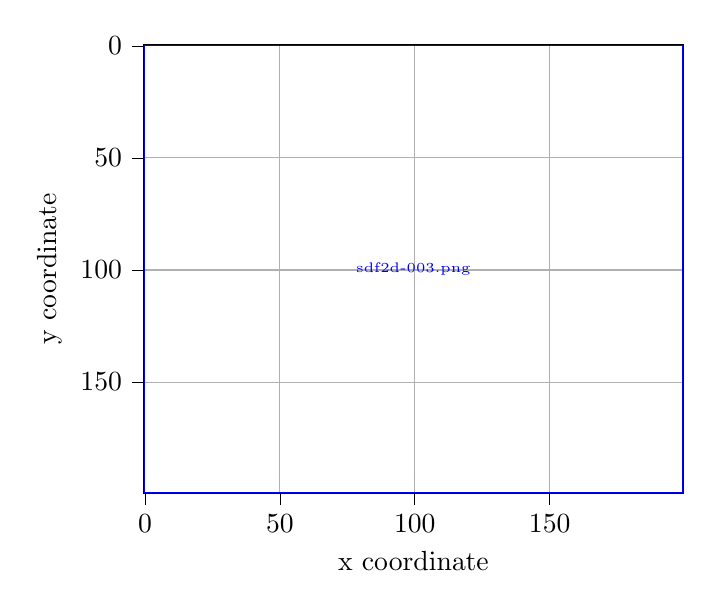
\begin{tikzpicture}

\begin{axis}[
tick align=outside,
tick pos=left,
x grid style={white!69.0196!black},
xlabel={x coordinate},
xmajorgrids,
xmin=-0.5000, xmax=199.5000,
xtick style={color=black},
y dir=reverse,
y grid style={white!69.0196!black},
ylabel={y coordinate},
ymajorgrids,
ymin=-0.5000, ymax=199.5000,
ytick style={color=black}
]
\addplot graphics [includegraphics cmd=\pgfimage,xmin=-0.5000, xmax=199.5000, ymin=199.5000, ymax=-0.5000] {sdf2d-003.png};
\end{axis}

\end{tikzpicture}

%         % % This file was created by tikzplotlib v0.9.1.
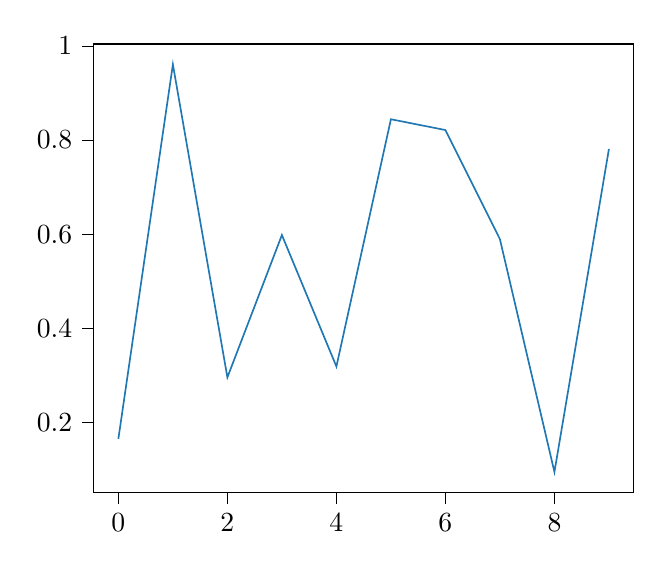
\begin{tikzpicture}

\definecolor{color0}{rgb}{0.12156862745098,0.466666666666667,0.705882352941177}

\begin{axis}[
tick align=outside,
tick pos=left,
x grid style={white!69.0196078431373!black},
xmin=-0.45, xmax=9.45,
xtick style={color=black},
y grid style={white!69.0196078431373!black},
ymin=0.0515297644926165, ymax=1.0037743262763,
ytick style={color=black}
]
\addplot [semithick, color0]
table {%
0 0.165204368712852
1 0.960490482558861
2 0.295706783168825
3 0.598084081751131
4 0.318814100655487
5 0.844017623549353
6 0.821076195130074
7 0.589191813076777
8 0.0948136082100567
9 0.781036863745426
};
\end{axis}

\end{tikzpicture}

%     \end{center}
%     \caption{a two dimensional SDF. $F(x,y) = \sqrt{x^2+y^2} - 1$} describes the unit circle.
% \end{figure}

Since the distance to the nearest surface is always known, the step size of a ray tracing algorithm can be dynamically adjusted, resulting in fewer iterations along a ray, see Figure \ref{sphereViz}..



\begin{figure}[ht]
\centerline{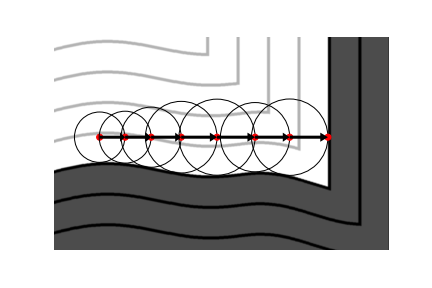
\includegraphics[scale=0.5]{img/sphereTracingViz.png}}
\caption{\label{sphereViz}{\it Visualization of the sphere tracing algorithm in 2D. A ray is sent from the source (left) to the right until it hits a surface, always moving the maximum distance as the SDF informs the tracing algorithm about the distance to nearest surface.}}
\end{figure}
%

% \begin{figure}
%     \begin{center}
%         %% Creator: Matplotlib, PGF backend
%%
%% To include the figure in your LaTeX document, write
%%   \input{<filename>.pgf}
%%
%% Make sure the required packages are loaded in your preamble
%%   \usepackage{pgf}
%%
%% Figures using additional raster images can only be included by \input if
%% they are in the same directory as the main LaTeX file. For loading figures
%% from other directories you can use the `import` package
%%   \usepackage{import}
%% and then include the figures with
%%   \import{<path to file>}{<filename>.pgf}
%%
%% Matplotlib used the following preamble
%%
\begingroup%
\makeatletter%
\begin{pgfpicture}%
\pgfpathrectangle{\pgfpointorigin}{\pgfqpoint{10.000000in}{10.000000in}}%
\pgfusepath{use as bounding box, clip}%
\begin{pgfscope}%
\pgfsetbuttcap%
\pgfsetmiterjoin%
\definecolor{currentfill}{rgb}{1.000000,1.000000,1.000000}%
\pgfsetfillcolor{currentfill}%
\pgfsetlinewidth{0.000000pt}%
\definecolor{currentstroke}{rgb}{1.000000,1.000000,1.000000}%
\pgfsetstrokecolor{currentstroke}%
\pgfsetdash{}{0pt}%
\pgfpathmoveto{\pgfqpoint{0.000000in}{0.000000in}}%
\pgfpathlineto{\pgfqpoint{10.000000in}{0.000000in}}%
\pgfpathlineto{\pgfqpoint{10.000000in}{10.000000in}}%
\pgfpathlineto{\pgfqpoint{0.000000in}{10.000000in}}%
\pgfpathclose%
\pgfusepath{fill}%
\end{pgfscope}%
\begin{pgfscope}%
\pgfsetbuttcap%
\pgfsetmiterjoin%
\definecolor{currentfill}{rgb}{1.000000,1.000000,1.000000}%
\pgfsetfillcolor{currentfill}%
\pgfsetlinewidth{0.000000pt}%
\definecolor{currentstroke}{rgb}{0.000000,0.000000,0.000000}%
\pgfsetstrokecolor{currentstroke}%
\pgfsetstrokeopacity{0.000000}%
\pgfsetdash{}{0pt}%
\pgfpathmoveto{\pgfqpoint{1.250000in}{2.559091in}}%
\pgfpathlineto{\pgfqpoint{9.000000in}{2.559091in}}%
\pgfpathlineto{\pgfqpoint{9.000000in}{7.490909in}}%
\pgfpathlineto{\pgfqpoint{1.250000in}{7.490909in}}%
\pgfpathclose%
\pgfusepath{fill}%
\end{pgfscope}%
\begin{pgfscope}%
\pgfpathrectangle{\pgfqpoint{1.250000in}{2.559091in}}{\pgfqpoint{7.750000in}{4.931818in}}%
\pgfusepath{clip}%
\pgfsys@transformshift{1.250000in}{2.559091in}%
\pgftext[left,bottom]{\pgfimage[interpolate=true,width=7.750000in,height=4.944444in]{sphereTracingViz-img0.png}}%
\end{pgfscope}%
\begin{pgfscope}%
\pgfpathrectangle{\pgfqpoint{1.250000in}{2.559091in}}{\pgfqpoint{7.750000in}{4.931818in}}%
\pgfusepath{clip}%
\pgfsetbuttcap%
\pgfsetmiterjoin%
\pgfsetlinewidth{1.003750pt}%
\definecolor{currentstroke}{rgb}{0.000000,0.000000,1.000000}%
\pgfsetstrokecolor{currentstroke}%
\pgfsetdash{}{0pt}%
\pgfpathmoveto{\pgfqpoint{2.306818in}{5.162386in}}%
\pgfpathcurveto{\pgfqpoint{2.307752in}{5.162386in}}{\pgfqpoint{2.308649in}{5.162758in}}{\pgfqpoint{2.309309in}{5.163418in}}%
\pgfpathcurveto{\pgfqpoint{2.309970in}{5.164079in}}{\pgfqpoint{2.310341in}{5.164975in}}{\pgfqpoint{2.310341in}{5.165909in}}%
\pgfpathcurveto{\pgfqpoint{2.310341in}{5.166843in}}{\pgfqpoint{2.309970in}{5.167739in}}{\pgfqpoint{2.309309in}{5.168400in}}%
\pgfpathcurveto{\pgfqpoint{2.308649in}{5.169061in}}{\pgfqpoint{2.307752in}{5.169432in}}{\pgfqpoint{2.306818in}{5.169432in}}%
\pgfpathcurveto{\pgfqpoint{2.305884in}{5.169432in}}{\pgfqpoint{2.304988in}{5.169061in}}{\pgfqpoint{2.304327in}{5.168400in}}%
\pgfpathcurveto{\pgfqpoint{2.303667in}{5.167739in}}{\pgfqpoint{2.303295in}{5.166843in}}{\pgfqpoint{2.303295in}{5.165909in}}%
\pgfpathcurveto{\pgfqpoint{2.303295in}{5.164975in}}{\pgfqpoint{2.303667in}{5.164079in}}{\pgfqpoint{2.304327in}{5.163418in}}%
\pgfpathcurveto{\pgfqpoint{2.304988in}{5.162758in}}{\pgfqpoint{2.305884in}{5.162386in}}{\pgfqpoint{2.306818in}{5.162386in}}%
\pgfpathclose%
\pgfusepath{stroke}%
\end{pgfscope}%
\begin{pgfscope}%
\pgfpathrectangle{\pgfqpoint{1.250000in}{2.559091in}}{\pgfqpoint{7.750000in}{4.931818in}}%
\pgfusepath{clip}%
\pgfsetbuttcap%
\pgfsetmiterjoin%
\pgfsetlinewidth{1.003750pt}%
\definecolor{currentstroke}{rgb}{0.000000,0.000000,0.000000}%
\pgfsetstrokecolor{currentstroke}%
\pgfsetdash{}{0pt}%
\pgfpathmoveto{\pgfqpoint{2.306818in}{4.582902in}}%
\pgfpathcurveto{\pgfqpoint{2.461434in}{4.582902in}}{\pgfqpoint{2.609737in}{4.644331in}}{\pgfqpoint{2.719067in}{4.753661in}}%
\pgfpathcurveto{\pgfqpoint{2.828396in}{4.862990in}}{\pgfqpoint{2.889826in}{5.011294in}}{\pgfqpoint{2.889826in}{5.165909in}}%
\pgfpathcurveto{\pgfqpoint{2.889826in}{5.320524in}}{\pgfqpoint{2.828396in}{5.468828in}}{\pgfqpoint{2.719067in}{5.578158in}}%
\pgfpathcurveto{\pgfqpoint{2.609737in}{5.687487in}}{\pgfqpoint{2.461434in}{5.748916in}}{\pgfqpoint{2.306818in}{5.748916in}}%
\pgfpathcurveto{\pgfqpoint{2.152203in}{5.748916in}}{\pgfqpoint{2.003899in}{5.687487in}}{\pgfqpoint{1.894570in}{5.578158in}}%
\pgfpathcurveto{\pgfqpoint{1.785240in}{5.468828in}}{\pgfqpoint{1.723811in}{5.320524in}}{\pgfqpoint{1.723811in}{5.165909in}}%
\pgfpathcurveto{\pgfqpoint{1.723811in}{5.011294in}}{\pgfqpoint{1.785240in}{4.862990in}}{\pgfqpoint{1.894570in}{4.753661in}}%
\pgfpathcurveto{\pgfqpoint{2.003899in}{4.644331in}}{\pgfqpoint{2.152203in}{4.582902in}}{\pgfqpoint{2.306818in}{4.582902in}}%
\pgfpathclose%
\pgfusepath{stroke}%
\end{pgfscope}%
\begin{pgfscope}%
\pgfpathrectangle{\pgfqpoint{1.250000in}{2.559091in}}{\pgfqpoint{7.750000in}{4.931818in}}%
\pgfusepath{clip}%
\pgfsetbuttcap%
\pgfsetmiterjoin%
\definecolor{currentfill}{rgb}{1.000000,0.000000,0.000000}%
\pgfsetfillcolor{currentfill}%
\pgfsetlinewidth{1.003750pt}%
\definecolor{currentstroke}{rgb}{1.000000,0.000000,0.000000}%
\pgfsetstrokecolor{currentstroke}%
\pgfsetdash{}{0pt}%
\pgfpathmoveto{\pgfqpoint{2.306818in}{5.095455in}}%
\pgfpathcurveto{\pgfqpoint{2.325503in}{5.095455in}}{\pgfqpoint{2.343425in}{5.102878in}}{\pgfqpoint{2.356637in}{5.116090in}}%
\pgfpathcurveto{\pgfqpoint{2.369849in}{5.129302in}}{\pgfqpoint{2.377273in}{5.147224in}}{\pgfqpoint{2.377273in}{5.165909in}}%
\pgfpathcurveto{\pgfqpoint{2.377273in}{5.184594in}}{\pgfqpoint{2.369849in}{5.202516in}}{\pgfqpoint{2.356637in}{5.215728in}}%
\pgfpathcurveto{\pgfqpoint{2.343425in}{5.228940in}}{\pgfqpoint{2.325503in}{5.236364in}}{\pgfqpoint{2.306818in}{5.236364in}}%
\pgfpathcurveto{\pgfqpoint{2.288133in}{5.236364in}}{\pgfqpoint{2.270211in}{5.228940in}}{\pgfqpoint{2.256999in}{5.215728in}}%
\pgfpathcurveto{\pgfqpoint{2.243787in}{5.202516in}}{\pgfqpoint{2.236364in}{5.184594in}}{\pgfqpoint{2.236364in}{5.165909in}}%
\pgfpathcurveto{\pgfqpoint{2.236364in}{5.147224in}}{\pgfqpoint{2.243787in}{5.129302in}}{\pgfqpoint{2.256999in}{5.116090in}}%
\pgfpathcurveto{\pgfqpoint{2.270211in}{5.102878in}}{\pgfqpoint{2.288133in}{5.095455in}}{\pgfqpoint{2.306818in}{5.095455in}}%
\pgfpathclose%
\pgfusepath{stroke,fill}%
\end{pgfscope}%
\begin{pgfscope}%
\pgfpathrectangle{\pgfqpoint{1.250000in}{2.559091in}}{\pgfqpoint{7.750000in}{4.931818in}}%
\pgfusepath{clip}%
\pgfsetbuttcap%
\pgfsetmiterjoin%
\definecolor{currentfill}{rgb}{0.000000,0.000000,0.000000}%
\pgfsetfillcolor{currentfill}%
\pgfsetlinewidth{0.000000pt}%
\definecolor{currentstroke}{rgb}{0.000000,0.000000,0.000000}%
\pgfsetstrokecolor{currentstroke}%
\pgfsetstrokeopacity{0.000000}%
\pgfsetdash{}{0pt}%
\pgfpathmoveto{\pgfqpoint{2.271591in}{5.165909in}}%
\pgfpathlineto{\pgfqpoint{2.342045in}{5.165909in}}%
\pgfpathlineto{\pgfqpoint{2.342045in}{5.165909in}}%
\pgfpathlineto{\pgfqpoint{2.412500in}{5.165909in}}%
\pgfpathlineto{\pgfqpoint{2.306818in}{5.165909in}}%
\pgfpathlineto{\pgfqpoint{2.201136in}{5.165909in}}%
\pgfpathlineto{\pgfqpoint{2.271591in}{5.165909in}}%
\pgfpathclose%
\pgfusepath{fill}%
\end{pgfscope}%
\begin{pgfscope}%
\pgfpathrectangle{\pgfqpoint{1.250000in}{2.559091in}}{\pgfqpoint{7.750000in}{4.931818in}}%
\pgfusepath{clip}%
\pgfsetbuttcap%
\pgfsetmiterjoin%
\pgfsetlinewidth{1.003750pt}%
\definecolor{currentstroke}{rgb}{0.000000,0.000000,0.000000}%
\pgfsetstrokecolor{currentstroke}%
\pgfsetdash{}{0pt}%
\pgfpathmoveto{\pgfqpoint{2.896871in}{4.564570in}}%
\pgfpathcurveto{\pgfqpoint{3.056348in}{4.564570in}}{\pgfqpoint{3.209315in}{4.627931in}}{\pgfqpoint{3.322082in}{4.740698in}}%
\pgfpathcurveto{\pgfqpoint{3.434849in}{4.853465in}}{\pgfqpoint{3.498210in}{5.006432in}}{\pgfqpoint{3.498210in}{5.165909in}}%
\pgfpathcurveto{\pgfqpoint{3.498210in}{5.325386in}}{\pgfqpoint{3.434849in}{5.478353in}}{\pgfqpoint{3.322082in}{5.591120in}}%
\pgfpathcurveto{\pgfqpoint{3.209315in}{5.703888in}}{\pgfqpoint{3.056348in}{5.767248in}}{\pgfqpoint{2.896871in}{5.767248in}}%
\pgfpathcurveto{\pgfqpoint{2.737394in}{5.767248in}}{\pgfqpoint{2.584427in}{5.703888in}}{\pgfqpoint{2.471660in}{5.591120in}}%
\pgfpathcurveto{\pgfqpoint{2.358893in}{5.478353in}}{\pgfqpoint{2.295532in}{5.325386in}}{\pgfqpoint{2.295532in}{5.165909in}}%
\pgfpathcurveto{\pgfqpoint{2.295532in}{5.006432in}}{\pgfqpoint{2.358893in}{4.853465in}}{\pgfqpoint{2.471660in}{4.740698in}}%
\pgfpathcurveto{\pgfqpoint{2.584427in}{4.627931in}}{\pgfqpoint{2.737394in}{4.564570in}}{\pgfqpoint{2.896871in}{4.564570in}}%
\pgfpathclose%
\pgfusepath{stroke}%
\end{pgfscope}%
\begin{pgfscope}%
\pgfpathrectangle{\pgfqpoint{1.250000in}{2.559091in}}{\pgfqpoint{7.750000in}{4.931818in}}%
\pgfusepath{clip}%
\pgfsetbuttcap%
\pgfsetmiterjoin%
\definecolor{currentfill}{rgb}{1.000000,0.000000,0.000000}%
\pgfsetfillcolor{currentfill}%
\pgfsetlinewidth{1.003750pt}%
\definecolor{currentstroke}{rgb}{1.000000,0.000000,0.000000}%
\pgfsetstrokecolor{currentstroke}%
\pgfsetdash{}{0pt}%
\pgfpathmoveto{\pgfqpoint{2.896871in}{5.095455in}}%
\pgfpathcurveto{\pgfqpoint{2.915556in}{5.095455in}}{\pgfqpoint{2.933478in}{5.102878in}}{\pgfqpoint{2.946690in}{5.116090in}}%
\pgfpathcurveto{\pgfqpoint{2.959902in}{5.129302in}}{\pgfqpoint{2.967326in}{5.147224in}}{\pgfqpoint{2.967326in}{5.165909in}}%
\pgfpathcurveto{\pgfqpoint{2.967326in}{5.184594in}}{\pgfqpoint{2.959902in}{5.202516in}}{\pgfqpoint{2.946690in}{5.215728in}}%
\pgfpathcurveto{\pgfqpoint{2.933478in}{5.228940in}}{\pgfqpoint{2.915556in}{5.236364in}}{\pgfqpoint{2.896871in}{5.236364in}}%
\pgfpathcurveto{\pgfqpoint{2.878186in}{5.236364in}}{\pgfqpoint{2.860264in}{5.228940in}}{\pgfqpoint{2.847052in}{5.215728in}}%
\pgfpathcurveto{\pgfqpoint{2.833840in}{5.202516in}}{\pgfqpoint{2.826416in}{5.184594in}}{\pgfqpoint{2.826416in}{5.165909in}}%
\pgfpathcurveto{\pgfqpoint{2.826416in}{5.147224in}}{\pgfqpoint{2.833840in}{5.129302in}}{\pgfqpoint{2.847052in}{5.116090in}}%
\pgfpathcurveto{\pgfqpoint{2.860264in}{5.102878in}}{\pgfqpoint{2.878186in}{5.095455in}}{\pgfqpoint{2.896871in}{5.095455in}}%
\pgfpathclose%
\pgfusepath{stroke,fill}%
\end{pgfscope}%
\begin{pgfscope}%
\pgfpathrectangle{\pgfqpoint{1.250000in}{2.559091in}}{\pgfqpoint{7.750000in}{4.931818in}}%
\pgfusepath{clip}%
\pgfsetbuttcap%
\pgfsetmiterjoin%
\definecolor{currentfill}{rgb}{0.000000,0.000000,0.000000}%
\pgfsetfillcolor{currentfill}%
\pgfsetlinewidth{0.000000pt}%
\definecolor{currentstroke}{rgb}{0.000000,0.000000,0.000000}%
\pgfsetstrokecolor{currentstroke}%
\pgfsetstrokeopacity{0.000000}%
\pgfsetdash{}{0pt}%
\pgfpathmoveto{\pgfqpoint{2.306818in}{5.201136in}}%
\pgfpathlineto{\pgfqpoint{2.306818in}{5.130682in}}%
\pgfpathlineto{\pgfqpoint{2.778860in}{5.130682in}}%
\pgfpathlineto{\pgfqpoint{2.778860in}{5.060227in}}%
\pgfpathlineto{\pgfqpoint{2.896871in}{5.165909in}}%
\pgfpathlineto{\pgfqpoint{2.778860in}{5.271591in}}%
\pgfpathlineto{\pgfqpoint{2.778860in}{5.201136in}}%
\pgfpathclose%
\pgfusepath{fill}%
\end{pgfscope}%
\begin{pgfscope}%
\pgfpathrectangle{\pgfqpoint{1.250000in}{2.559091in}}{\pgfqpoint{7.750000in}{4.931818in}}%
\pgfusepath{clip}%
\pgfsetbuttcap%
\pgfsetmiterjoin%
\pgfsetlinewidth{1.003750pt}%
\definecolor{currentstroke}{rgb}{0.000000,0.000000,0.000000}%
\pgfsetstrokecolor{currentstroke}%
\pgfsetdash{}{0pt}%
\pgfpathmoveto{\pgfqpoint{3.498210in}{4.469585in}}%
\pgfpathcurveto{\pgfqpoint{3.682878in}{4.469585in}}{\pgfqpoint{3.860007in}{4.542954in}}{\pgfqpoint{3.990586in}{4.673533in}}%
\pgfpathcurveto{\pgfqpoint{4.121166in}{4.804113in}}{\pgfqpoint{4.194535in}{4.981242in}}{\pgfqpoint{4.194535in}{5.165909in}}%
\pgfpathcurveto{\pgfqpoint{4.194535in}{5.350576in}}{\pgfqpoint{4.121166in}{5.527705in}}{\pgfqpoint{3.990586in}{5.658285in}}%
\pgfpathcurveto{\pgfqpoint{3.860007in}{5.788864in}}{\pgfqpoint{3.682878in}{5.862234in}}{\pgfqpoint{3.498210in}{5.862234in}}%
\pgfpathcurveto{\pgfqpoint{3.313543in}{5.862234in}}{\pgfqpoint{3.136414in}{5.788864in}}{\pgfqpoint{3.005835in}{5.658285in}}%
\pgfpathcurveto{\pgfqpoint{2.875255in}{5.527705in}}{\pgfqpoint{2.801886in}{5.350576in}}{\pgfqpoint{2.801886in}{5.165909in}}%
\pgfpathcurveto{\pgfqpoint{2.801886in}{4.981242in}}{\pgfqpoint{2.875255in}{4.804113in}}{\pgfqpoint{3.005835in}{4.673533in}}%
\pgfpathcurveto{\pgfqpoint{3.136414in}{4.542954in}}{\pgfqpoint{3.313543in}{4.469585in}}{\pgfqpoint{3.498210in}{4.469585in}}%
\pgfpathclose%
\pgfusepath{stroke}%
\end{pgfscope}%
\begin{pgfscope}%
\pgfpathrectangle{\pgfqpoint{1.250000in}{2.559091in}}{\pgfqpoint{7.750000in}{4.931818in}}%
\pgfusepath{clip}%
\pgfsetbuttcap%
\pgfsetmiterjoin%
\definecolor{currentfill}{rgb}{1.000000,0.000000,0.000000}%
\pgfsetfillcolor{currentfill}%
\pgfsetlinewidth{1.003750pt}%
\definecolor{currentstroke}{rgb}{1.000000,0.000000,0.000000}%
\pgfsetstrokecolor{currentstroke}%
\pgfsetdash{}{0pt}%
\pgfpathmoveto{\pgfqpoint{3.498210in}{5.095455in}}%
\pgfpathcurveto{\pgfqpoint{3.516895in}{5.095455in}}{\pgfqpoint{3.534817in}{5.102878in}}{\pgfqpoint{3.548029in}{5.116090in}}%
\pgfpathcurveto{\pgfqpoint{3.561241in}{5.129302in}}{\pgfqpoint{3.568665in}{5.147224in}}{\pgfqpoint{3.568665in}{5.165909in}}%
\pgfpathcurveto{\pgfqpoint{3.568665in}{5.184594in}}{\pgfqpoint{3.561241in}{5.202516in}}{\pgfqpoint{3.548029in}{5.215728in}}%
\pgfpathcurveto{\pgfqpoint{3.534817in}{5.228940in}}{\pgfqpoint{3.516895in}{5.236364in}}{\pgfqpoint{3.498210in}{5.236364in}}%
\pgfpathcurveto{\pgfqpoint{3.479526in}{5.236364in}}{\pgfqpoint{3.461604in}{5.228940in}}{\pgfqpoint{3.448392in}{5.215728in}}%
\pgfpathcurveto{\pgfqpoint{3.435179in}{5.202516in}}{\pgfqpoint{3.427756in}{5.184594in}}{\pgfqpoint{3.427756in}{5.165909in}}%
\pgfpathcurveto{\pgfqpoint{3.427756in}{5.147224in}}{\pgfqpoint{3.435179in}{5.129302in}}{\pgfqpoint{3.448392in}{5.116090in}}%
\pgfpathcurveto{\pgfqpoint{3.461604in}{5.102878in}}{\pgfqpoint{3.479526in}{5.095455in}}{\pgfqpoint{3.498210in}{5.095455in}}%
\pgfpathclose%
\pgfusepath{stroke,fill}%
\end{pgfscope}%
\begin{pgfscope}%
\pgfpathrectangle{\pgfqpoint{1.250000in}{2.559091in}}{\pgfqpoint{7.750000in}{4.931818in}}%
\pgfusepath{clip}%
\pgfsetbuttcap%
\pgfsetmiterjoin%
\definecolor{currentfill}{rgb}{0.000000,0.000000,0.000000}%
\pgfsetfillcolor{currentfill}%
\pgfsetlinewidth{0.000000pt}%
\definecolor{currentstroke}{rgb}{0.000000,0.000000,0.000000}%
\pgfsetstrokecolor{currentstroke}%
\pgfsetstrokeopacity{0.000000}%
\pgfsetdash{}{0pt}%
\pgfpathmoveto{\pgfqpoint{2.896871in}{5.201136in}}%
\pgfpathlineto{\pgfqpoint{2.896871in}{5.130682in}}%
\pgfpathlineto{\pgfqpoint{3.377943in}{5.130682in}}%
\pgfpathlineto{\pgfqpoint{3.377943in}{5.060227in}}%
\pgfpathlineto{\pgfqpoint{3.498210in}{5.165909in}}%
\pgfpathlineto{\pgfqpoint{3.377943in}{5.271591in}}%
\pgfpathlineto{\pgfqpoint{3.377943in}{5.201136in}}%
\pgfpathclose%
\pgfusepath{fill}%
\end{pgfscope}%
\begin{pgfscope}%
\pgfpathrectangle{\pgfqpoint{1.250000in}{2.559091in}}{\pgfqpoint{7.750000in}{4.931818in}}%
\pgfusepath{clip}%
\pgfsetbuttcap%
\pgfsetmiterjoin%
\pgfsetlinewidth{1.003750pt}%
\definecolor{currentstroke}{rgb}{0.000000,0.000000,0.000000}%
\pgfsetstrokecolor{currentstroke}%
\pgfsetdash{}{0pt}%
\pgfpathmoveto{\pgfqpoint{4.194535in}{4.336603in}}%
\pgfpathcurveto{\pgfqpoint{4.414469in}{4.336603in}}{\pgfqpoint{4.625426in}{4.423984in}}{\pgfqpoint{4.780943in}{4.579501in}}%
\pgfpathcurveto{\pgfqpoint{4.936460in}{4.735018in}}{\pgfqpoint{5.023841in}{4.945974in}}{\pgfqpoint{5.023841in}{5.165909in}}%
\pgfpathcurveto{\pgfqpoint{5.023841in}{5.385844in}}{\pgfqpoint{4.936460in}{5.596800in}}{\pgfqpoint{4.780943in}{5.752317in}}%
\pgfpathcurveto{\pgfqpoint{4.625426in}{5.907834in}}{\pgfqpoint{4.414469in}{5.995215in}}{\pgfqpoint{4.194535in}{5.995215in}}%
\pgfpathcurveto{\pgfqpoint{3.974600in}{5.995215in}}{\pgfqpoint{3.763644in}{5.907834in}}{\pgfqpoint{3.608127in}{5.752317in}}%
\pgfpathcurveto{\pgfqpoint{3.452609in}{5.596800in}}{\pgfqpoint{3.365228in}{5.385844in}}{\pgfqpoint{3.365228in}{5.165909in}}%
\pgfpathcurveto{\pgfqpoint{3.365228in}{4.945974in}}{\pgfqpoint{3.452609in}{4.735018in}}{\pgfqpoint{3.608127in}{4.579501in}}%
\pgfpathcurveto{\pgfqpoint{3.763644in}{4.423984in}}{\pgfqpoint{3.974600in}{4.336603in}}{\pgfqpoint{4.194535in}{4.336603in}}%
\pgfpathclose%
\pgfusepath{stroke}%
\end{pgfscope}%
\begin{pgfscope}%
\pgfpathrectangle{\pgfqpoint{1.250000in}{2.559091in}}{\pgfqpoint{7.750000in}{4.931818in}}%
\pgfusepath{clip}%
\pgfsetbuttcap%
\pgfsetmiterjoin%
\definecolor{currentfill}{rgb}{1.000000,0.000000,0.000000}%
\pgfsetfillcolor{currentfill}%
\pgfsetlinewidth{1.003750pt}%
\definecolor{currentstroke}{rgb}{1.000000,0.000000,0.000000}%
\pgfsetstrokecolor{currentstroke}%
\pgfsetdash{}{0pt}%
\pgfpathmoveto{\pgfqpoint{4.194535in}{5.095455in}}%
\pgfpathcurveto{\pgfqpoint{4.213220in}{5.095455in}}{\pgfqpoint{4.231142in}{5.102878in}}{\pgfqpoint{4.244354in}{5.116090in}}%
\pgfpathcurveto{\pgfqpoint{4.257566in}{5.129302in}}{\pgfqpoint{4.264989in}{5.147224in}}{\pgfqpoint{4.264989in}{5.165909in}}%
\pgfpathcurveto{\pgfqpoint{4.264989in}{5.184594in}}{\pgfqpoint{4.257566in}{5.202516in}}{\pgfqpoint{4.244354in}{5.215728in}}%
\pgfpathcurveto{\pgfqpoint{4.231142in}{5.228940in}}{\pgfqpoint{4.213220in}{5.236364in}}{\pgfqpoint{4.194535in}{5.236364in}}%
\pgfpathcurveto{\pgfqpoint{4.175850in}{5.236364in}}{\pgfqpoint{4.157928in}{5.228940in}}{\pgfqpoint{4.144716in}{5.215728in}}%
\pgfpathcurveto{\pgfqpoint{4.131504in}{5.202516in}}{\pgfqpoint{4.124080in}{5.184594in}}{\pgfqpoint{4.124080in}{5.165909in}}%
\pgfpathcurveto{\pgfqpoint{4.124080in}{5.147224in}}{\pgfqpoint{4.131504in}{5.129302in}}{\pgfqpoint{4.144716in}{5.116090in}}%
\pgfpathcurveto{\pgfqpoint{4.157928in}{5.102878in}}{\pgfqpoint{4.175850in}{5.095455in}}{\pgfqpoint{4.194535in}{5.095455in}}%
\pgfpathclose%
\pgfusepath{stroke,fill}%
\end{pgfscope}%
\begin{pgfscope}%
\pgfpathrectangle{\pgfqpoint{1.250000in}{2.559091in}}{\pgfqpoint{7.750000in}{4.931818in}}%
\pgfusepath{clip}%
\pgfsetbuttcap%
\pgfsetmiterjoin%
\definecolor{currentfill}{rgb}{0.000000,0.000000,0.000000}%
\pgfsetfillcolor{currentfill}%
\pgfsetlinewidth{0.000000pt}%
\definecolor{currentstroke}{rgb}{0.000000,0.000000,0.000000}%
\pgfsetstrokecolor{currentstroke}%
\pgfsetstrokeopacity{0.000000}%
\pgfsetdash{}{0pt}%
\pgfpathmoveto{\pgfqpoint{3.498210in}{5.201136in}}%
\pgfpathlineto{\pgfqpoint{3.498210in}{5.130682in}}%
\pgfpathlineto{\pgfqpoint{4.055270in}{5.130682in}}%
\pgfpathlineto{\pgfqpoint{4.055270in}{5.060227in}}%
\pgfpathlineto{\pgfqpoint{4.194535in}{5.165909in}}%
\pgfpathlineto{\pgfqpoint{4.055270in}{5.271591in}}%
\pgfpathlineto{\pgfqpoint{4.055270in}{5.201136in}}%
\pgfpathclose%
\pgfusepath{fill}%
\end{pgfscope}%
\begin{pgfscope}%
\pgfpathrectangle{\pgfqpoint{1.250000in}{2.559091in}}{\pgfqpoint{7.750000in}{4.931818in}}%
\pgfusepath{clip}%
\pgfsetbuttcap%
\pgfsetmiterjoin%
\pgfsetlinewidth{1.003750pt}%
\definecolor{currentstroke}{rgb}{0.000000,0.000000,0.000000}%
\pgfsetstrokecolor{currentstroke}%
\pgfsetdash{}{0pt}%
\pgfpathmoveto{\pgfqpoint{5.023841in}{4.285127in}}%
\pgfpathcurveto{\pgfqpoint{5.257427in}{4.285127in}}{\pgfqpoint{5.481478in}{4.377931in}}{\pgfqpoint{5.646648in}{4.543102in}}%
\pgfpathcurveto{\pgfqpoint{5.811819in}{4.708272in}}{\pgfqpoint{5.904624in}{4.932323in}}{\pgfqpoint{5.904624in}{5.165909in}}%
\pgfpathcurveto{\pgfqpoint{5.904624in}{5.399495in}}{\pgfqpoint{5.811819in}{5.623546in}}{\pgfqpoint{5.646648in}{5.788716in}}%
\pgfpathcurveto{\pgfqpoint{5.481478in}{5.953887in}}{\pgfqpoint{5.257427in}{6.046692in}}{\pgfqpoint{5.023841in}{6.046692in}}%
\pgfpathcurveto{\pgfqpoint{4.790255in}{6.046692in}}{\pgfqpoint{4.566204in}{5.953887in}}{\pgfqpoint{4.401034in}{5.788716in}}%
\pgfpathcurveto{\pgfqpoint{4.235864in}{5.623546in}}{\pgfqpoint{4.143059in}{5.399495in}}{\pgfqpoint{4.143059in}{5.165909in}}%
\pgfpathcurveto{\pgfqpoint{4.143059in}{4.932323in}}{\pgfqpoint{4.235864in}{4.708272in}}{\pgfqpoint{4.401034in}{4.543102in}}%
\pgfpathcurveto{\pgfqpoint{4.566204in}{4.377931in}}{\pgfqpoint{4.790255in}{4.285127in}}{\pgfqpoint{5.023841in}{4.285127in}}%
\pgfpathclose%
\pgfusepath{stroke}%
\end{pgfscope}%
\begin{pgfscope}%
\pgfpathrectangle{\pgfqpoint{1.250000in}{2.559091in}}{\pgfqpoint{7.750000in}{4.931818in}}%
\pgfusepath{clip}%
\pgfsetbuttcap%
\pgfsetmiterjoin%
\definecolor{currentfill}{rgb}{1.000000,0.000000,0.000000}%
\pgfsetfillcolor{currentfill}%
\pgfsetlinewidth{1.003750pt}%
\definecolor{currentstroke}{rgb}{1.000000,0.000000,0.000000}%
\pgfsetstrokecolor{currentstroke}%
\pgfsetdash{}{0pt}%
\pgfpathmoveto{\pgfqpoint{5.023841in}{5.095455in}}%
\pgfpathcurveto{\pgfqpoint{5.042526in}{5.095455in}}{\pgfqpoint{5.060448in}{5.102878in}}{\pgfqpoint{5.073660in}{5.116090in}}%
\pgfpathcurveto{\pgfqpoint{5.086872in}{5.129302in}}{\pgfqpoint{5.094296in}{5.147224in}}{\pgfqpoint{5.094296in}{5.165909in}}%
\pgfpathcurveto{\pgfqpoint{5.094296in}{5.184594in}}{\pgfqpoint{5.086872in}{5.202516in}}{\pgfqpoint{5.073660in}{5.215728in}}%
\pgfpathcurveto{\pgfqpoint{5.060448in}{5.228940in}}{\pgfqpoint{5.042526in}{5.236364in}}{\pgfqpoint{5.023841in}{5.236364in}}%
\pgfpathcurveto{\pgfqpoint{5.005156in}{5.236364in}}{\pgfqpoint{4.987234in}{5.228940in}}{\pgfqpoint{4.974022in}{5.215728in}}%
\pgfpathcurveto{\pgfqpoint{4.960810in}{5.202516in}}{\pgfqpoint{4.953387in}{5.184594in}}{\pgfqpoint{4.953387in}{5.165909in}}%
\pgfpathcurveto{\pgfqpoint{4.953387in}{5.147224in}}{\pgfqpoint{4.960810in}{5.129302in}}{\pgfqpoint{4.974022in}{5.116090in}}%
\pgfpathcurveto{\pgfqpoint{4.987234in}{5.102878in}}{\pgfqpoint{5.005156in}{5.095455in}}{\pgfqpoint{5.023841in}{5.095455in}}%
\pgfpathclose%
\pgfusepath{stroke,fill}%
\end{pgfscope}%
\begin{pgfscope}%
\pgfpathrectangle{\pgfqpoint{1.250000in}{2.559091in}}{\pgfqpoint{7.750000in}{4.931818in}}%
\pgfusepath{clip}%
\pgfsetbuttcap%
\pgfsetmiterjoin%
\definecolor{currentfill}{rgb}{0.000000,0.000000,0.000000}%
\pgfsetfillcolor{currentfill}%
\pgfsetlinewidth{0.000000pt}%
\definecolor{currentstroke}{rgb}{0.000000,0.000000,0.000000}%
\pgfsetstrokecolor{currentstroke}%
\pgfsetstrokeopacity{0.000000}%
\pgfsetdash{}{0pt}%
\pgfpathmoveto{\pgfqpoint{4.194535in}{5.201136in}}%
\pgfpathlineto{\pgfqpoint{4.194535in}{5.130682in}}%
\pgfpathlineto{\pgfqpoint{4.857980in}{5.130682in}}%
\pgfpathlineto{\pgfqpoint{4.857980in}{5.060227in}}%
\pgfpathlineto{\pgfqpoint{5.023841in}{5.165909in}}%
\pgfpathlineto{\pgfqpoint{4.857980in}{5.271591in}}%
\pgfpathlineto{\pgfqpoint{4.857980in}{5.201136in}}%
\pgfpathclose%
\pgfusepath{fill}%
\end{pgfscope}%
\begin{pgfscope}%
\pgfpathrectangle{\pgfqpoint{1.250000in}{2.559091in}}{\pgfqpoint{7.750000in}{4.931818in}}%
\pgfusepath{clip}%
\pgfsetbuttcap%
\pgfsetmiterjoin%
\pgfsetlinewidth{1.003750pt}%
\definecolor{currentstroke}{rgb}{0.000000,0.000000,0.000000}%
\pgfsetstrokecolor{currentstroke}%
\pgfsetdash{}{0pt}%
\pgfpathmoveto{\pgfqpoint{5.904624in}{4.363898in}}%
\pgfpathcurveto{\pgfqpoint{6.117320in}{4.363898in}}{\pgfqpoint{6.321333in}{4.448403in}}{\pgfqpoint{6.471732in}{4.598801in}}%
\pgfpathcurveto{\pgfqpoint{6.622130in}{4.749200in}}{\pgfqpoint{6.706635in}{4.953213in}}{\pgfqpoint{6.706635in}{5.165909in}}%
\pgfpathcurveto{\pgfqpoint{6.706635in}{5.378605in}}{\pgfqpoint{6.622130in}{5.582618in}}{\pgfqpoint{6.471732in}{5.733017in}}%
\pgfpathcurveto{\pgfqpoint{6.321333in}{5.883416in}}{\pgfqpoint{6.117320in}{5.967921in}}{\pgfqpoint{5.904624in}{5.967921in}}%
\pgfpathcurveto{\pgfqpoint{5.691928in}{5.967921in}}{\pgfqpoint{5.487915in}{5.883416in}}{\pgfqpoint{5.337516in}{5.733017in}}%
\pgfpathcurveto{\pgfqpoint{5.187117in}{5.582618in}}{\pgfqpoint{5.102612in}{5.378605in}}{\pgfqpoint{5.102612in}{5.165909in}}%
\pgfpathcurveto{\pgfqpoint{5.102612in}{4.953213in}}{\pgfqpoint{5.187117in}{4.749200in}}{\pgfqpoint{5.337516in}{4.598801in}}%
\pgfpathcurveto{\pgfqpoint{5.487915in}{4.448403in}}{\pgfqpoint{5.691928in}{4.363898in}}{\pgfqpoint{5.904624in}{4.363898in}}%
\pgfpathclose%
\pgfusepath{stroke}%
\end{pgfscope}%
\begin{pgfscope}%
\pgfpathrectangle{\pgfqpoint{1.250000in}{2.559091in}}{\pgfqpoint{7.750000in}{4.931818in}}%
\pgfusepath{clip}%
\pgfsetbuttcap%
\pgfsetmiterjoin%
\definecolor{currentfill}{rgb}{1.000000,0.000000,0.000000}%
\pgfsetfillcolor{currentfill}%
\pgfsetlinewidth{1.003750pt}%
\definecolor{currentstroke}{rgb}{1.000000,0.000000,0.000000}%
\pgfsetstrokecolor{currentstroke}%
\pgfsetdash{}{0pt}%
\pgfpathmoveto{\pgfqpoint{5.904624in}{5.095455in}}%
\pgfpathcurveto{\pgfqpoint{5.923308in}{5.095455in}}{\pgfqpoint{5.941230in}{5.102878in}}{\pgfqpoint{5.954443in}{5.116090in}}%
\pgfpathcurveto{\pgfqpoint{5.967655in}{5.129302in}}{\pgfqpoint{5.975078in}{5.147224in}}{\pgfqpoint{5.975078in}{5.165909in}}%
\pgfpathcurveto{\pgfqpoint{5.975078in}{5.184594in}}{\pgfqpoint{5.967655in}{5.202516in}}{\pgfqpoint{5.954443in}{5.215728in}}%
\pgfpathcurveto{\pgfqpoint{5.941230in}{5.228940in}}{\pgfqpoint{5.923308in}{5.236364in}}{\pgfqpoint{5.904624in}{5.236364in}}%
\pgfpathcurveto{\pgfqpoint{5.885939in}{5.236364in}}{\pgfqpoint{5.868017in}{5.228940in}}{\pgfqpoint{5.854805in}{5.215728in}}%
\pgfpathcurveto{\pgfqpoint{5.841593in}{5.202516in}}{\pgfqpoint{5.834169in}{5.184594in}}{\pgfqpoint{5.834169in}{5.165909in}}%
\pgfpathcurveto{\pgfqpoint{5.834169in}{5.147224in}}{\pgfqpoint{5.841593in}{5.129302in}}{\pgfqpoint{5.854805in}{5.116090in}}%
\pgfpathcurveto{\pgfqpoint{5.868017in}{5.102878in}}{\pgfqpoint{5.885939in}{5.095455in}}{\pgfqpoint{5.904624in}{5.095455in}}%
\pgfpathclose%
\pgfusepath{stroke,fill}%
\end{pgfscope}%
\begin{pgfscope}%
\pgfpathrectangle{\pgfqpoint{1.250000in}{2.559091in}}{\pgfqpoint{7.750000in}{4.931818in}}%
\pgfusepath{clip}%
\pgfsetbuttcap%
\pgfsetmiterjoin%
\definecolor{currentfill}{rgb}{0.000000,0.000000,0.000000}%
\pgfsetfillcolor{currentfill}%
\pgfsetlinewidth{0.000000pt}%
\definecolor{currentstroke}{rgb}{0.000000,0.000000,0.000000}%
\pgfsetstrokecolor{currentstroke}%
\pgfsetstrokeopacity{0.000000}%
\pgfsetdash{}{0pt}%
\pgfpathmoveto{\pgfqpoint{5.023841in}{5.201136in}}%
\pgfpathlineto{\pgfqpoint{5.023841in}{5.130682in}}%
\pgfpathlineto{\pgfqpoint{5.728467in}{5.130682in}}%
\pgfpathlineto{\pgfqpoint{5.728467in}{5.060227in}}%
\pgfpathlineto{\pgfqpoint{5.904624in}{5.165909in}}%
\pgfpathlineto{\pgfqpoint{5.728467in}{5.271591in}}%
\pgfpathlineto{\pgfqpoint{5.728467in}{5.201136in}}%
\pgfpathclose%
\pgfusepath{fill}%
\end{pgfscope}%
\begin{pgfscope}%
\pgfpathrectangle{\pgfqpoint{1.250000in}{2.559091in}}{\pgfqpoint{7.750000in}{4.931818in}}%
\pgfusepath{clip}%
\pgfsetbuttcap%
\pgfsetmiterjoin%
\pgfsetlinewidth{1.003750pt}%
\definecolor{currentstroke}{rgb}{0.000000,0.000000,0.000000}%
\pgfsetstrokecolor{currentstroke}%
\pgfsetdash{}{0pt}%
\pgfpathmoveto{\pgfqpoint{6.706635in}{4.281635in}}%
\pgfpathcurveto{\pgfqpoint{6.941147in}{4.281635in}}{\pgfqpoint{7.166086in}{4.374808in}}{\pgfqpoint{7.331911in}{4.540633in}}%
\pgfpathcurveto{\pgfqpoint{7.497736in}{4.706458in}}{\pgfqpoint{7.590909in}{4.931397in}}{\pgfqpoint{7.590909in}{5.165909in}}%
\pgfpathcurveto{\pgfqpoint{7.590909in}{5.400421in}}{\pgfqpoint{7.497736in}{5.625360in}}{\pgfqpoint{7.331911in}{5.791185in}}%
\pgfpathcurveto{\pgfqpoint{7.166086in}{5.957010in}}{\pgfqpoint{6.941147in}{6.050183in}}{\pgfqpoint{6.706635in}{6.050183in}}%
\pgfpathcurveto{\pgfqpoint{6.472123in}{6.050183in}}{\pgfqpoint{6.247184in}{5.957010in}}{\pgfqpoint{6.081359in}{5.791185in}}%
\pgfpathcurveto{\pgfqpoint{5.915534in}{5.625360in}}{\pgfqpoint{5.822361in}{5.400421in}}{\pgfqpoint{5.822361in}{5.165909in}}%
\pgfpathcurveto{\pgfqpoint{5.822361in}{4.931397in}}{\pgfqpoint{5.915534in}{4.706458in}}{\pgfqpoint{6.081359in}{4.540633in}}%
\pgfpathcurveto{\pgfqpoint{6.247184in}{4.374808in}}{\pgfqpoint{6.472123in}{4.281635in}}{\pgfqpoint{6.706635in}{4.281635in}}%
\pgfpathclose%
\pgfusepath{stroke}%
\end{pgfscope}%
\begin{pgfscope}%
\pgfpathrectangle{\pgfqpoint{1.250000in}{2.559091in}}{\pgfqpoint{7.750000in}{4.931818in}}%
\pgfusepath{clip}%
\pgfsetbuttcap%
\pgfsetmiterjoin%
\definecolor{currentfill}{rgb}{1.000000,0.000000,0.000000}%
\pgfsetfillcolor{currentfill}%
\pgfsetlinewidth{1.003750pt}%
\definecolor{currentstroke}{rgb}{1.000000,0.000000,0.000000}%
\pgfsetstrokecolor{currentstroke}%
\pgfsetdash{}{0pt}%
\pgfpathmoveto{\pgfqpoint{6.706635in}{5.095455in}}%
\pgfpathcurveto{\pgfqpoint{6.725320in}{5.095455in}}{\pgfqpoint{6.743242in}{5.102878in}}{\pgfqpoint{6.756454in}{5.116090in}}%
\pgfpathcurveto{\pgfqpoint{6.769666in}{5.129302in}}{\pgfqpoint{6.777090in}{5.147224in}}{\pgfqpoint{6.777090in}{5.165909in}}%
\pgfpathcurveto{\pgfqpoint{6.777090in}{5.184594in}}{\pgfqpoint{6.769666in}{5.202516in}}{\pgfqpoint{6.756454in}{5.215728in}}%
\pgfpathcurveto{\pgfqpoint{6.743242in}{5.228940in}}{\pgfqpoint{6.725320in}{5.236364in}}{\pgfqpoint{6.706635in}{5.236364in}}%
\pgfpathcurveto{\pgfqpoint{6.687951in}{5.236364in}}{\pgfqpoint{6.670029in}{5.228940in}}{\pgfqpoint{6.656816in}{5.215728in}}%
\pgfpathcurveto{\pgfqpoint{6.643604in}{5.202516in}}{\pgfqpoint{6.636181in}{5.184594in}}{\pgfqpoint{6.636181in}{5.165909in}}%
\pgfpathcurveto{\pgfqpoint{6.636181in}{5.147224in}}{\pgfqpoint{6.643604in}{5.129302in}}{\pgfqpoint{6.656816in}{5.116090in}}%
\pgfpathcurveto{\pgfqpoint{6.670029in}{5.102878in}}{\pgfqpoint{6.687951in}{5.095455in}}{\pgfqpoint{6.706635in}{5.095455in}}%
\pgfpathclose%
\pgfusepath{stroke,fill}%
\end{pgfscope}%
\begin{pgfscope}%
\pgfpathrectangle{\pgfqpoint{1.250000in}{2.559091in}}{\pgfqpoint{7.750000in}{4.931818in}}%
\pgfusepath{clip}%
\pgfsetbuttcap%
\pgfsetmiterjoin%
\definecolor{currentfill}{rgb}{0.000000,0.000000,0.000000}%
\pgfsetfillcolor{currentfill}%
\pgfsetlinewidth{0.000000pt}%
\definecolor{currentstroke}{rgb}{0.000000,0.000000,0.000000}%
\pgfsetstrokecolor{currentstroke}%
\pgfsetstrokeopacity{0.000000}%
\pgfsetdash{}{0pt}%
\pgfpathmoveto{\pgfqpoint{5.904624in}{5.201136in}}%
\pgfpathlineto{\pgfqpoint{5.904624in}{5.130682in}}%
\pgfpathlineto{\pgfqpoint{6.546233in}{5.130682in}}%
\pgfpathlineto{\pgfqpoint{6.546233in}{5.060227in}}%
\pgfpathlineto{\pgfqpoint{6.706635in}{5.165909in}}%
\pgfpathlineto{\pgfqpoint{6.546233in}{5.271591in}}%
\pgfpathlineto{\pgfqpoint{6.546233in}{5.201136in}}%
\pgfpathclose%
\pgfusepath{fill}%
\end{pgfscope}%
\begin{pgfscope}%
\pgfpathrectangle{\pgfqpoint{1.250000in}{2.559091in}}{\pgfqpoint{7.750000in}{4.931818in}}%
\pgfusepath{clip}%
\pgfsetbuttcap%
\pgfsetmiterjoin%
\pgfsetlinewidth{1.003750pt}%
\definecolor{currentstroke}{rgb}{0.000000,0.000000,0.000000}%
\pgfsetstrokecolor{currentstroke}%
\pgfsetdash{}{0pt}%
\pgfpathmoveto{\pgfqpoint{7.590909in}{5.165909in}}%
\pgfpathcurveto{\pgfqpoint{7.590909in}{5.165909in}}{\pgfqpoint{7.590909in}{5.165909in}}{\pgfqpoint{7.590909in}{5.165909in}}%
\pgfpathcurveto{\pgfqpoint{7.590909in}{5.165909in}}{\pgfqpoint{7.590909in}{5.165909in}}{\pgfqpoint{7.590909in}{5.165909in}}%
\pgfpathcurveto{\pgfqpoint{7.590909in}{5.165909in}}{\pgfqpoint{7.590909in}{5.165909in}}{\pgfqpoint{7.590909in}{5.165909in}}%
\pgfpathcurveto{\pgfqpoint{7.590909in}{5.165909in}}{\pgfqpoint{7.590909in}{5.165909in}}{\pgfqpoint{7.590909in}{5.165909in}}%
\pgfpathcurveto{\pgfqpoint{7.590909in}{5.165909in}}{\pgfqpoint{7.590909in}{5.165909in}}{\pgfqpoint{7.590909in}{5.165909in}}%
\pgfpathcurveto{\pgfqpoint{7.590909in}{5.165909in}}{\pgfqpoint{7.590909in}{5.165909in}}{\pgfqpoint{7.590909in}{5.165909in}}%
\pgfpathcurveto{\pgfqpoint{7.590909in}{5.165909in}}{\pgfqpoint{7.590909in}{5.165909in}}{\pgfqpoint{7.590909in}{5.165909in}}%
\pgfpathcurveto{\pgfqpoint{7.590909in}{5.165909in}}{\pgfqpoint{7.590909in}{5.165909in}}{\pgfqpoint{7.590909in}{5.165909in}}%
\pgfpathclose%
\pgfusepath{stroke}%
\end{pgfscope}%
\begin{pgfscope}%
\pgfpathrectangle{\pgfqpoint{1.250000in}{2.559091in}}{\pgfqpoint{7.750000in}{4.931818in}}%
\pgfusepath{clip}%
\pgfsetbuttcap%
\pgfsetmiterjoin%
\definecolor{currentfill}{rgb}{1.000000,0.000000,0.000000}%
\pgfsetfillcolor{currentfill}%
\pgfsetlinewidth{1.003750pt}%
\definecolor{currentstroke}{rgb}{1.000000,0.000000,0.000000}%
\pgfsetstrokecolor{currentstroke}%
\pgfsetdash{}{0pt}%
\pgfpathmoveto{\pgfqpoint{7.590909in}{5.095455in}}%
\pgfpathcurveto{\pgfqpoint{7.609594in}{5.095455in}}{\pgfqpoint{7.627516in}{5.102878in}}{\pgfqpoint{7.640728in}{5.116090in}}%
\pgfpathcurveto{\pgfqpoint{7.653940in}{5.129302in}}{\pgfqpoint{7.661364in}{5.147224in}}{\pgfqpoint{7.661364in}{5.165909in}}%
\pgfpathcurveto{\pgfqpoint{7.661364in}{5.184594in}}{\pgfqpoint{7.653940in}{5.202516in}}{\pgfqpoint{7.640728in}{5.215728in}}%
\pgfpathcurveto{\pgfqpoint{7.627516in}{5.228940in}}{\pgfqpoint{7.609594in}{5.236364in}}{\pgfqpoint{7.590909in}{5.236364in}}%
\pgfpathcurveto{\pgfqpoint{7.572224in}{5.236364in}}{\pgfqpoint{7.554302in}{5.228940in}}{\pgfqpoint{7.541090in}{5.215728in}}%
\pgfpathcurveto{\pgfqpoint{7.527878in}{5.202516in}}{\pgfqpoint{7.520455in}{5.184594in}}{\pgfqpoint{7.520455in}{5.165909in}}%
\pgfpathcurveto{\pgfqpoint{7.520455in}{5.147224in}}{\pgfqpoint{7.527878in}{5.129302in}}{\pgfqpoint{7.541090in}{5.116090in}}%
\pgfpathcurveto{\pgfqpoint{7.554302in}{5.102878in}}{\pgfqpoint{7.572224in}{5.095455in}}{\pgfqpoint{7.590909in}{5.095455in}}%
\pgfpathclose%
\pgfusepath{stroke,fill}%
\end{pgfscope}%
\begin{pgfscope}%
\pgfpathrectangle{\pgfqpoint{1.250000in}{2.559091in}}{\pgfqpoint{7.750000in}{4.931818in}}%
\pgfusepath{clip}%
\pgfsetbuttcap%
\pgfsetmiterjoin%
\definecolor{currentfill}{rgb}{0.000000,0.000000,0.000000}%
\pgfsetfillcolor{currentfill}%
\pgfsetlinewidth{0.000000pt}%
\definecolor{currentstroke}{rgb}{0.000000,0.000000,0.000000}%
\pgfsetstrokecolor{currentstroke}%
\pgfsetstrokeopacity{0.000000}%
\pgfsetdash{}{0pt}%
\pgfpathmoveto{\pgfqpoint{6.706635in}{5.201136in}}%
\pgfpathlineto{\pgfqpoint{6.706635in}{5.130682in}}%
\pgfpathlineto{\pgfqpoint{7.414054in}{5.130682in}}%
\pgfpathlineto{\pgfqpoint{7.414054in}{5.060227in}}%
\pgfpathlineto{\pgfqpoint{7.590909in}{5.165909in}}%
\pgfpathlineto{\pgfqpoint{7.414054in}{5.271591in}}%
\pgfpathlineto{\pgfqpoint{7.414054in}{5.201136in}}%
\pgfpathclose%
\pgfusepath{fill}%
\end{pgfscope}%
\begin{pgfscope}%
\pgfsetbuttcap%
\pgfsetroundjoin%
\definecolor{currentfill}{rgb}{0.000000,0.000000,0.000000}%
\pgfsetfillcolor{currentfill}%
\pgfsetlinewidth{0.803000pt}%
\definecolor{currentstroke}{rgb}{0.000000,0.000000,0.000000}%
\pgfsetstrokecolor{currentstroke}%
\pgfsetdash{}{0pt}%
\pgfsys@defobject{currentmarker}{\pgfqpoint{0.000000in}{-0.048611in}}{\pgfqpoint{0.000000in}{0.000000in}}{%
\pgfpathmoveto{\pgfqpoint{0.000000in}{0.000000in}}%
\pgfpathlineto{\pgfqpoint{0.000000in}{-0.048611in}}%
\pgfusepath{stroke,fill}%
}%
\begin{pgfscope}%
\pgfsys@transformshift{1.250000in}{2.559091in}%
\pgfsys@useobject{currentmarker}{}%
\end{pgfscope}%
\end{pgfscope}%
\begin{pgfscope}%
\definecolor{textcolor}{rgb}{0.000000,0.000000,0.000000}%
\pgfsetstrokecolor{textcolor}%
\pgfsetfillcolor{textcolor}%
\pgftext[x=1.250000in,y=2.461869in,,top]{\color{textcolor}\rmfamily\fontsize{10.000000}{12.000000}\selectfont \(\displaystyle 400\)}%
\end{pgfscope}%
\begin{pgfscope}%
\pgfsetbuttcap%
\pgfsetroundjoin%
\definecolor{currentfill}{rgb}{0.000000,0.000000,0.000000}%
\pgfsetfillcolor{currentfill}%
\pgfsetlinewidth{0.803000pt}%
\definecolor{currentstroke}{rgb}{0.000000,0.000000,0.000000}%
\pgfsetstrokecolor{currentstroke}%
\pgfsetdash{}{0pt}%
\pgfsys@defobject{currentmarker}{\pgfqpoint{0.000000in}{-0.048611in}}{\pgfqpoint{0.000000in}{0.000000in}}{%
\pgfpathmoveto{\pgfqpoint{0.000000in}{0.000000in}}%
\pgfpathlineto{\pgfqpoint{0.000000in}{-0.048611in}}%
\pgfusepath{stroke,fill}%
}%
\begin{pgfscope}%
\pgfsys@transformshift{2.659091in}{2.559091in}%
\pgfsys@useobject{currentmarker}{}%
\end{pgfscope}%
\end{pgfscope}%
\begin{pgfscope}%
\definecolor{textcolor}{rgb}{0.000000,0.000000,0.000000}%
\pgfsetstrokecolor{textcolor}%
\pgfsetfillcolor{textcolor}%
\pgftext[x=2.659091in,y=2.461869in,,top]{\color{textcolor}\rmfamily\fontsize{10.000000}{12.000000}\selectfont \(\displaystyle 600\)}%
\end{pgfscope}%
\begin{pgfscope}%
\pgfsetbuttcap%
\pgfsetroundjoin%
\definecolor{currentfill}{rgb}{0.000000,0.000000,0.000000}%
\pgfsetfillcolor{currentfill}%
\pgfsetlinewidth{0.803000pt}%
\definecolor{currentstroke}{rgb}{0.000000,0.000000,0.000000}%
\pgfsetstrokecolor{currentstroke}%
\pgfsetdash{}{0pt}%
\pgfsys@defobject{currentmarker}{\pgfqpoint{0.000000in}{-0.048611in}}{\pgfqpoint{0.000000in}{0.000000in}}{%
\pgfpathmoveto{\pgfqpoint{0.000000in}{0.000000in}}%
\pgfpathlineto{\pgfqpoint{0.000000in}{-0.048611in}}%
\pgfusepath{stroke,fill}%
}%
\begin{pgfscope}%
\pgfsys@transformshift{4.068182in}{2.559091in}%
\pgfsys@useobject{currentmarker}{}%
\end{pgfscope}%
\end{pgfscope}%
\begin{pgfscope}%
\definecolor{textcolor}{rgb}{0.000000,0.000000,0.000000}%
\pgfsetstrokecolor{textcolor}%
\pgfsetfillcolor{textcolor}%
\pgftext[x=4.068182in,y=2.461869in,,top]{\color{textcolor}\rmfamily\fontsize{10.000000}{12.000000}\selectfont \(\displaystyle 800\)}%
\end{pgfscope}%
\begin{pgfscope}%
\pgfsetbuttcap%
\pgfsetroundjoin%
\definecolor{currentfill}{rgb}{0.000000,0.000000,0.000000}%
\pgfsetfillcolor{currentfill}%
\pgfsetlinewidth{0.803000pt}%
\definecolor{currentstroke}{rgb}{0.000000,0.000000,0.000000}%
\pgfsetstrokecolor{currentstroke}%
\pgfsetdash{}{0pt}%
\pgfsys@defobject{currentmarker}{\pgfqpoint{0.000000in}{-0.048611in}}{\pgfqpoint{0.000000in}{0.000000in}}{%
\pgfpathmoveto{\pgfqpoint{0.000000in}{0.000000in}}%
\pgfpathlineto{\pgfqpoint{0.000000in}{-0.048611in}}%
\pgfusepath{stroke,fill}%
}%
\begin{pgfscope}%
\pgfsys@transformshift{5.477273in}{2.559091in}%
\pgfsys@useobject{currentmarker}{}%
\end{pgfscope}%
\end{pgfscope}%
\begin{pgfscope}%
\definecolor{textcolor}{rgb}{0.000000,0.000000,0.000000}%
\pgfsetstrokecolor{textcolor}%
\pgfsetfillcolor{textcolor}%
\pgftext[x=5.477273in,y=2.461869in,,top]{\color{textcolor}\rmfamily\fontsize{10.000000}{12.000000}\selectfont \(\displaystyle 1000\)}%
\end{pgfscope}%
\begin{pgfscope}%
\pgfsetbuttcap%
\pgfsetroundjoin%
\definecolor{currentfill}{rgb}{0.000000,0.000000,0.000000}%
\pgfsetfillcolor{currentfill}%
\pgfsetlinewidth{0.803000pt}%
\definecolor{currentstroke}{rgb}{0.000000,0.000000,0.000000}%
\pgfsetstrokecolor{currentstroke}%
\pgfsetdash{}{0pt}%
\pgfsys@defobject{currentmarker}{\pgfqpoint{0.000000in}{-0.048611in}}{\pgfqpoint{0.000000in}{0.000000in}}{%
\pgfpathmoveto{\pgfqpoint{0.000000in}{0.000000in}}%
\pgfpathlineto{\pgfqpoint{0.000000in}{-0.048611in}}%
\pgfusepath{stroke,fill}%
}%
\begin{pgfscope}%
\pgfsys@transformshift{6.886364in}{2.559091in}%
\pgfsys@useobject{currentmarker}{}%
\end{pgfscope}%
\end{pgfscope}%
\begin{pgfscope}%
\definecolor{textcolor}{rgb}{0.000000,0.000000,0.000000}%
\pgfsetstrokecolor{textcolor}%
\pgfsetfillcolor{textcolor}%
\pgftext[x=6.886364in,y=2.461869in,,top]{\color{textcolor}\rmfamily\fontsize{10.000000}{12.000000}\selectfont \(\displaystyle 1200\)}%
\end{pgfscope}%
\begin{pgfscope}%
\pgfsetbuttcap%
\pgfsetroundjoin%
\definecolor{currentfill}{rgb}{0.000000,0.000000,0.000000}%
\pgfsetfillcolor{currentfill}%
\pgfsetlinewidth{0.803000pt}%
\definecolor{currentstroke}{rgb}{0.000000,0.000000,0.000000}%
\pgfsetstrokecolor{currentstroke}%
\pgfsetdash{}{0pt}%
\pgfsys@defobject{currentmarker}{\pgfqpoint{0.000000in}{-0.048611in}}{\pgfqpoint{0.000000in}{0.000000in}}{%
\pgfpathmoveto{\pgfqpoint{0.000000in}{0.000000in}}%
\pgfpathlineto{\pgfqpoint{0.000000in}{-0.048611in}}%
\pgfusepath{stroke,fill}%
}%
\begin{pgfscope}%
\pgfsys@transformshift{8.295455in}{2.559091in}%
\pgfsys@useobject{currentmarker}{}%
\end{pgfscope}%
\end{pgfscope}%
\begin{pgfscope}%
\definecolor{textcolor}{rgb}{0.000000,0.000000,0.000000}%
\pgfsetstrokecolor{textcolor}%
\pgfsetfillcolor{textcolor}%
\pgftext[x=8.295455in,y=2.461869in,,top]{\color{textcolor}\rmfamily\fontsize{10.000000}{12.000000}\selectfont \(\displaystyle 1400\)}%
\end{pgfscope}%
\begin{pgfscope}%
\definecolor{textcolor}{rgb}{0.000000,0.000000,0.000000}%
\pgfsetstrokecolor{textcolor}%
\pgfsetfillcolor{textcolor}%
\pgftext[x=5.125000in,y=2.282856in,,top]{\color{textcolor}\rmfamily\fontsize{10.000000}{12.000000}\selectfont x coordinate}%
\end{pgfscope}%
\begin{pgfscope}%
\pgfsetbuttcap%
\pgfsetroundjoin%
\definecolor{currentfill}{rgb}{0.000000,0.000000,0.000000}%
\pgfsetfillcolor{currentfill}%
\pgfsetlinewidth{0.803000pt}%
\definecolor{currentstroke}{rgb}{0.000000,0.000000,0.000000}%
\pgfsetstrokecolor{currentstroke}%
\pgfsetdash{}{0pt}%
\pgfsys@defobject{currentmarker}{\pgfqpoint{-0.048611in}{0.000000in}}{\pgfqpoint{0.000000in}{0.000000in}}{%
\pgfpathmoveto{\pgfqpoint{0.000000in}{0.000000in}}%
\pgfpathlineto{\pgfqpoint{-0.048611in}{0.000000in}}%
\pgfusepath{stroke,fill}%
}%
\begin{pgfscope}%
\pgfsys@transformshift{1.250000in}{2.559091in}%
\pgfsys@useobject{currentmarker}{}%
\end{pgfscope}%
\end{pgfscope}%
\begin{pgfscope}%
\definecolor{textcolor}{rgb}{0.000000,0.000000,0.000000}%
\pgfsetstrokecolor{textcolor}%
\pgfsetfillcolor{textcolor}%
\pgftext[x=0.944444in,y=2.510866in,left,base]{\color{textcolor}\rmfamily\fontsize{10.000000}{12.000000}\selectfont \(\displaystyle 500\)}%
\end{pgfscope}%
\begin{pgfscope}%
\pgfsetbuttcap%
\pgfsetroundjoin%
\definecolor{currentfill}{rgb}{0.000000,0.000000,0.000000}%
\pgfsetfillcolor{currentfill}%
\pgfsetlinewidth{0.803000pt}%
\definecolor{currentstroke}{rgb}{0.000000,0.000000,0.000000}%
\pgfsetstrokecolor{currentstroke}%
\pgfsetdash{}{0pt}%
\pgfsys@defobject{currentmarker}{\pgfqpoint{-0.048611in}{0.000000in}}{\pgfqpoint{0.000000in}{0.000000in}}{%
\pgfpathmoveto{\pgfqpoint{0.000000in}{0.000000in}}%
\pgfpathlineto{\pgfqpoint{-0.048611in}{0.000000in}}%
\pgfusepath{stroke,fill}%
}%
\begin{pgfscope}%
\pgfsys@transformshift{1.250000in}{3.263636in}%
\pgfsys@useobject{currentmarker}{}%
\end{pgfscope}%
\end{pgfscope}%
\begin{pgfscope}%
\definecolor{textcolor}{rgb}{0.000000,0.000000,0.000000}%
\pgfsetstrokecolor{textcolor}%
\pgfsetfillcolor{textcolor}%
\pgftext[x=0.944444in,y=3.215411in,left,base]{\color{textcolor}\rmfamily\fontsize{10.000000}{12.000000}\selectfont \(\displaystyle 600\)}%
\end{pgfscope}%
\begin{pgfscope}%
\pgfsetbuttcap%
\pgfsetroundjoin%
\definecolor{currentfill}{rgb}{0.000000,0.000000,0.000000}%
\pgfsetfillcolor{currentfill}%
\pgfsetlinewidth{0.803000pt}%
\definecolor{currentstroke}{rgb}{0.000000,0.000000,0.000000}%
\pgfsetstrokecolor{currentstroke}%
\pgfsetdash{}{0pt}%
\pgfsys@defobject{currentmarker}{\pgfqpoint{-0.048611in}{0.000000in}}{\pgfqpoint{0.000000in}{0.000000in}}{%
\pgfpathmoveto{\pgfqpoint{0.000000in}{0.000000in}}%
\pgfpathlineto{\pgfqpoint{-0.048611in}{0.000000in}}%
\pgfusepath{stroke,fill}%
}%
\begin{pgfscope}%
\pgfsys@transformshift{1.250000in}{3.968182in}%
\pgfsys@useobject{currentmarker}{}%
\end{pgfscope}%
\end{pgfscope}%
\begin{pgfscope}%
\definecolor{textcolor}{rgb}{0.000000,0.000000,0.000000}%
\pgfsetstrokecolor{textcolor}%
\pgfsetfillcolor{textcolor}%
\pgftext[x=0.944444in,y=3.919957in,left,base]{\color{textcolor}\rmfamily\fontsize{10.000000}{12.000000}\selectfont \(\displaystyle 700\)}%
\end{pgfscope}%
\begin{pgfscope}%
\pgfsetbuttcap%
\pgfsetroundjoin%
\definecolor{currentfill}{rgb}{0.000000,0.000000,0.000000}%
\pgfsetfillcolor{currentfill}%
\pgfsetlinewidth{0.803000pt}%
\definecolor{currentstroke}{rgb}{0.000000,0.000000,0.000000}%
\pgfsetstrokecolor{currentstroke}%
\pgfsetdash{}{0pt}%
\pgfsys@defobject{currentmarker}{\pgfqpoint{-0.048611in}{0.000000in}}{\pgfqpoint{0.000000in}{0.000000in}}{%
\pgfpathmoveto{\pgfqpoint{0.000000in}{0.000000in}}%
\pgfpathlineto{\pgfqpoint{-0.048611in}{0.000000in}}%
\pgfusepath{stroke,fill}%
}%
\begin{pgfscope}%
\pgfsys@transformshift{1.250000in}{4.672727in}%
\pgfsys@useobject{currentmarker}{}%
\end{pgfscope}%
\end{pgfscope}%
\begin{pgfscope}%
\definecolor{textcolor}{rgb}{0.000000,0.000000,0.000000}%
\pgfsetstrokecolor{textcolor}%
\pgfsetfillcolor{textcolor}%
\pgftext[x=0.944444in,y=4.624502in,left,base]{\color{textcolor}\rmfamily\fontsize{10.000000}{12.000000}\selectfont \(\displaystyle 800\)}%
\end{pgfscope}%
\begin{pgfscope}%
\pgfsetbuttcap%
\pgfsetroundjoin%
\definecolor{currentfill}{rgb}{0.000000,0.000000,0.000000}%
\pgfsetfillcolor{currentfill}%
\pgfsetlinewidth{0.803000pt}%
\definecolor{currentstroke}{rgb}{0.000000,0.000000,0.000000}%
\pgfsetstrokecolor{currentstroke}%
\pgfsetdash{}{0pt}%
\pgfsys@defobject{currentmarker}{\pgfqpoint{-0.048611in}{0.000000in}}{\pgfqpoint{0.000000in}{0.000000in}}{%
\pgfpathmoveto{\pgfqpoint{0.000000in}{0.000000in}}%
\pgfpathlineto{\pgfqpoint{-0.048611in}{0.000000in}}%
\pgfusepath{stroke,fill}%
}%
\begin{pgfscope}%
\pgfsys@transformshift{1.250000in}{5.377273in}%
\pgfsys@useobject{currentmarker}{}%
\end{pgfscope}%
\end{pgfscope}%
\begin{pgfscope}%
\definecolor{textcolor}{rgb}{0.000000,0.000000,0.000000}%
\pgfsetstrokecolor{textcolor}%
\pgfsetfillcolor{textcolor}%
\pgftext[x=0.944444in,y=5.329047in,left,base]{\color{textcolor}\rmfamily\fontsize{10.000000}{12.000000}\selectfont \(\displaystyle 900\)}%
\end{pgfscope}%
\begin{pgfscope}%
\pgfsetbuttcap%
\pgfsetroundjoin%
\definecolor{currentfill}{rgb}{0.000000,0.000000,0.000000}%
\pgfsetfillcolor{currentfill}%
\pgfsetlinewidth{0.803000pt}%
\definecolor{currentstroke}{rgb}{0.000000,0.000000,0.000000}%
\pgfsetstrokecolor{currentstroke}%
\pgfsetdash{}{0pt}%
\pgfsys@defobject{currentmarker}{\pgfqpoint{-0.048611in}{0.000000in}}{\pgfqpoint{0.000000in}{0.000000in}}{%
\pgfpathmoveto{\pgfqpoint{0.000000in}{0.000000in}}%
\pgfpathlineto{\pgfqpoint{-0.048611in}{0.000000in}}%
\pgfusepath{stroke,fill}%
}%
\begin{pgfscope}%
\pgfsys@transformshift{1.250000in}{6.081818in}%
\pgfsys@useobject{currentmarker}{}%
\end{pgfscope}%
\end{pgfscope}%
\begin{pgfscope}%
\definecolor{textcolor}{rgb}{0.000000,0.000000,0.000000}%
\pgfsetstrokecolor{textcolor}%
\pgfsetfillcolor{textcolor}%
\pgftext[x=0.874999in,y=6.033593in,left,base]{\color{textcolor}\rmfamily\fontsize{10.000000}{12.000000}\selectfont \(\displaystyle 1000\)}%
\end{pgfscope}%
\begin{pgfscope}%
\pgfsetbuttcap%
\pgfsetroundjoin%
\definecolor{currentfill}{rgb}{0.000000,0.000000,0.000000}%
\pgfsetfillcolor{currentfill}%
\pgfsetlinewidth{0.803000pt}%
\definecolor{currentstroke}{rgb}{0.000000,0.000000,0.000000}%
\pgfsetstrokecolor{currentstroke}%
\pgfsetdash{}{0pt}%
\pgfsys@defobject{currentmarker}{\pgfqpoint{-0.048611in}{0.000000in}}{\pgfqpoint{0.000000in}{0.000000in}}{%
\pgfpathmoveto{\pgfqpoint{0.000000in}{0.000000in}}%
\pgfpathlineto{\pgfqpoint{-0.048611in}{0.000000in}}%
\pgfusepath{stroke,fill}%
}%
\begin{pgfscope}%
\pgfsys@transformshift{1.250000in}{6.786364in}%
\pgfsys@useobject{currentmarker}{}%
\end{pgfscope}%
\end{pgfscope}%
\begin{pgfscope}%
\definecolor{textcolor}{rgb}{0.000000,0.000000,0.000000}%
\pgfsetstrokecolor{textcolor}%
\pgfsetfillcolor{textcolor}%
\pgftext[x=0.874999in,y=6.738138in,left,base]{\color{textcolor}\rmfamily\fontsize{10.000000}{12.000000}\selectfont \(\displaystyle 1100\)}%
\end{pgfscope}%
\begin{pgfscope}%
\pgfsetbuttcap%
\pgfsetroundjoin%
\definecolor{currentfill}{rgb}{0.000000,0.000000,0.000000}%
\pgfsetfillcolor{currentfill}%
\pgfsetlinewidth{0.803000pt}%
\definecolor{currentstroke}{rgb}{0.000000,0.000000,0.000000}%
\pgfsetstrokecolor{currentstroke}%
\pgfsetdash{}{0pt}%
\pgfsys@defobject{currentmarker}{\pgfqpoint{-0.048611in}{0.000000in}}{\pgfqpoint{0.000000in}{0.000000in}}{%
\pgfpathmoveto{\pgfqpoint{0.000000in}{0.000000in}}%
\pgfpathlineto{\pgfqpoint{-0.048611in}{0.000000in}}%
\pgfusepath{stroke,fill}%
}%
\begin{pgfscope}%
\pgfsys@transformshift{1.250000in}{7.490909in}%
\pgfsys@useobject{currentmarker}{}%
\end{pgfscope}%
\end{pgfscope}%
\begin{pgfscope}%
\definecolor{textcolor}{rgb}{0.000000,0.000000,0.000000}%
\pgfsetstrokecolor{textcolor}%
\pgfsetfillcolor{textcolor}%
\pgftext[x=0.874999in,y=7.442684in,left,base]{\color{textcolor}\rmfamily\fontsize{10.000000}{12.000000}\selectfont \(\displaystyle 1200\)}%
\end{pgfscope}%
\begin{pgfscope}%
\definecolor{textcolor}{rgb}{0.000000,0.000000,0.000000}%
\pgfsetstrokecolor{textcolor}%
\pgfsetfillcolor{textcolor}%
\pgftext[x=0.819444in,y=5.025000in,,bottom,rotate=90.000000]{\color{textcolor}\rmfamily\fontsize{10.000000}{12.000000}\selectfont y coordinate}%
\end{pgfscope}%
\begin{pgfscope}%
\pgfsetrectcap%
\pgfsetmiterjoin%
\pgfsetlinewidth{0.803000pt}%
\definecolor{currentstroke}{rgb}{0.000000,0.000000,0.000000}%
\pgfsetstrokecolor{currentstroke}%
\pgfsetdash{}{0pt}%
\pgfpathmoveto{\pgfqpoint{1.250000in}{2.559091in}}%
\pgfpathlineto{\pgfqpoint{1.250000in}{7.490909in}}%
\pgfusepath{stroke}%
\end{pgfscope}%
\begin{pgfscope}%
\pgfsetrectcap%
\pgfsetmiterjoin%
\pgfsetlinewidth{0.803000pt}%
\definecolor{currentstroke}{rgb}{0.000000,0.000000,0.000000}%
\pgfsetstrokecolor{currentstroke}%
\pgfsetdash{}{0pt}%
\pgfpathmoveto{\pgfqpoint{9.000000in}{2.559091in}}%
\pgfpathlineto{\pgfqpoint{9.000000in}{7.490909in}}%
\pgfusepath{stroke}%
\end{pgfscope}%
\begin{pgfscope}%
\pgfsetrectcap%
\pgfsetmiterjoin%
\pgfsetlinewidth{0.803000pt}%
\definecolor{currentstroke}{rgb}{0.000000,0.000000,0.000000}%
\pgfsetstrokecolor{currentstroke}%
\pgfsetdash{}{0pt}%
\pgfpathmoveto{\pgfqpoint{1.250000in}{2.559091in}}%
\pgfpathlineto{\pgfqpoint{9.000000in}{2.559091in}}%
\pgfusepath{stroke}%
\end{pgfscope}%
\begin{pgfscope}%
\pgfsetrectcap%
\pgfsetmiterjoin%
\pgfsetlinewidth{0.803000pt}%
\definecolor{currentstroke}{rgb}{0.000000,0.000000,0.000000}%
\pgfsetstrokecolor{currentstroke}%
\pgfsetdash{}{0pt}%
\pgfpathmoveto{\pgfqpoint{1.250000in}{7.490909in}}%
\pgfpathlineto{\pgfqpoint{9.000000in}{7.490909in}}%
\pgfusepath{stroke}%
\end{pgfscope}%
\end{pgfpicture}%
\makeatother%
\endgroup%

%     \end{center}
%     \caption{A PGF histogram from \texttt{matplotlib}.}
% \end{figure}


% This enables the technique of sphere tracing, which has been used extensively in the so called demo scene to render impressive 3D video demos in real time for decades. 


% \begin{figure}[ht]
% \centerline{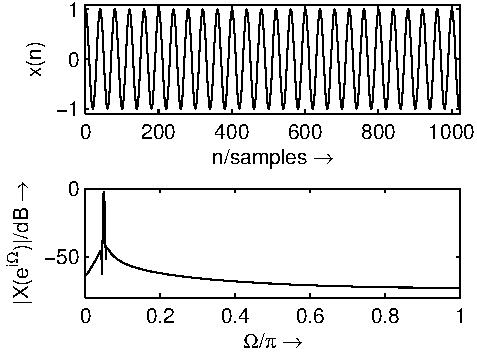
\includegraphics[scale=0.8]{fft_plot2}}
% \caption{\label{fft_plot}{\it Sinusoid in time and frequency domain. Short captions are centred, long captions (more than 1 line) are justified.}}
% \end{figure}


\subsection{Previous Work}
\label{ssec:prev}
A lot of previous work exists both in the field of Ray/sphere tracing and RIR estimation.
As shown in \cite{alpkocak_computing_2010} and \cite{brinkmann_round_2019} there are numerous approaches for estimating RIRs. 
NVIDIA is working in the field of real time ray traced audio simulation
NVIDIA VRWorks™ Audio (introduced with the Pascal GPU architecture) 

\cite{cao_interactive_2016} bidirectional ray tracing.

\subsubsection*{RIR Estimation}
\cite{alpkocak_computing_2010} gives an overview of methods in use for RIR estimation.

image source method, wave based, ray tracing.


\subsubsection*{Sphere Tracing}

Defining SDFs is an active field of research and there are several projects that aim at easier construction of SDFs and integration in 3D frameworks such as \href{https://github.com/Flafla2/Generic-Raymarch-Unity}{https://github.com/Flafla2/Generic-Raymarch-Unity} and \cite{lechner_hrtlacektdraymarchtoolkit_2020}.



\subsection{Motivation}
The reasons why sphere tracing in a compute shader for RIR estimation has not been documented until now probably lie in the relatively new introduction of compute shaders as well as in the difficulty of creating SDFs(in comparison to using existing 3D /CAD models and import them to polygon based ray tracers).
\subsubsection{Sphere tracing}
As described above, ray tracing in general is in use. Sphere tracing has a number of advantages over ray tracing polygonal surfaces. It is "procedural" by default, since all geometry is defined by implicit surface equations. More over sphere tracing approximates cone tracing for reducing aliasing artifacts in the pixel domain\cite{hart_sphere_1996}, which in the audio domain, is considered to have advantages but is very time confusing in a non-SDF setup\cite{alpkocak_computing_2010}. The deformation and rounding of geometry is possible in a very efficient way, which might offer an opportunity to approximate low-frequency response due to diffraction artifacts. Since geometry is not defined via vertizes and edges, there is no such thing as increasing the complexity of a shape in this way. Rounding a geometrical shape is a mere subtraction since it just shifts the rendering to another iso-surface, which is getting increasingly smooth as shown in \ref{sdf_2d_box}. Depending on the construction of the geometry, this way, holes and cavities (such as in a diffusor) can also be made disappear for a low-frequency pass as shown in figure \ref{fig:diffSmooth}.

\begin{figure}[ht]
\centerline{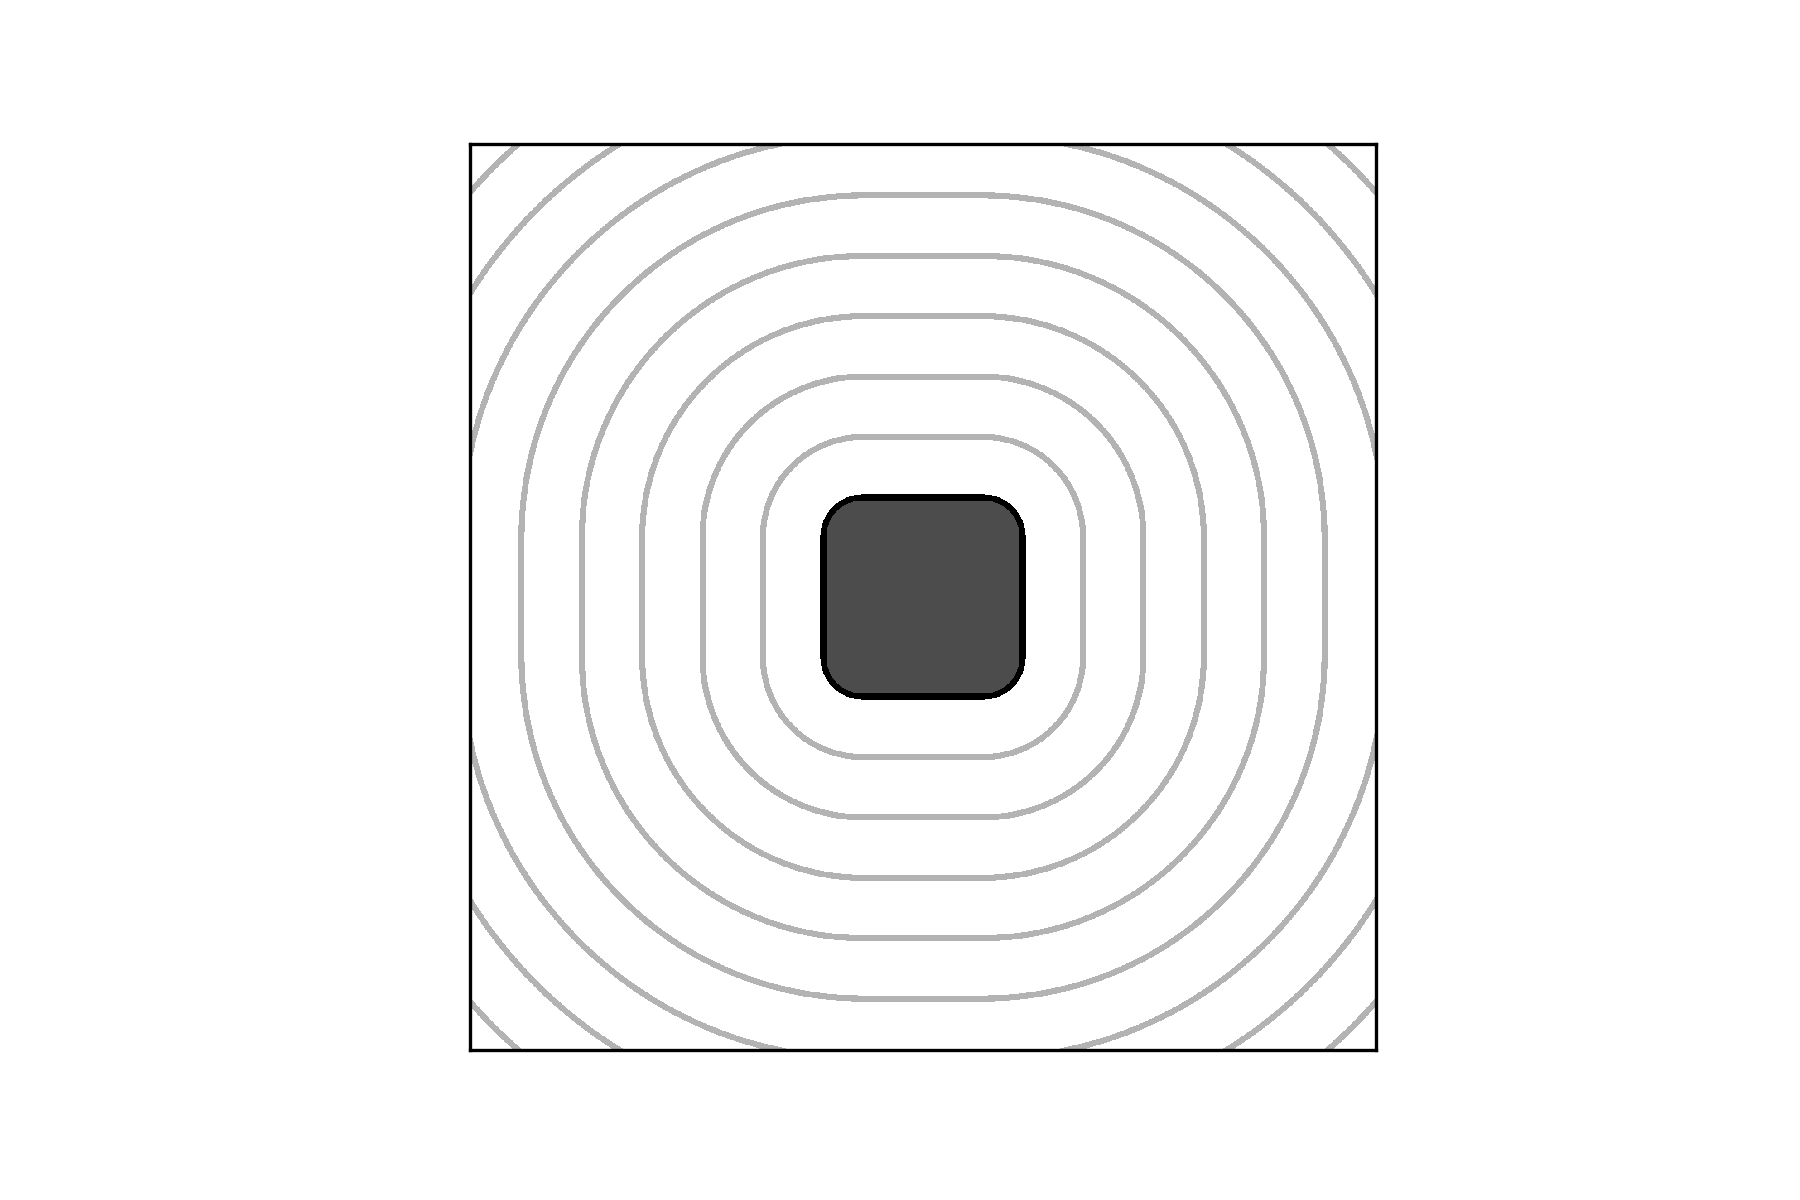
\includegraphics[scale=0.6]{img/sdf2dbox.png}}
\caption{\label{sdf_2d_box}{\it rounding the box given in Equation \ref{eq1} by subtraction of $0.7$.}}
\end{figure}  



\begin{figure}[ht]
\centering
\begin{subfigure}[t]{0.2\textwidth}
  \centering
  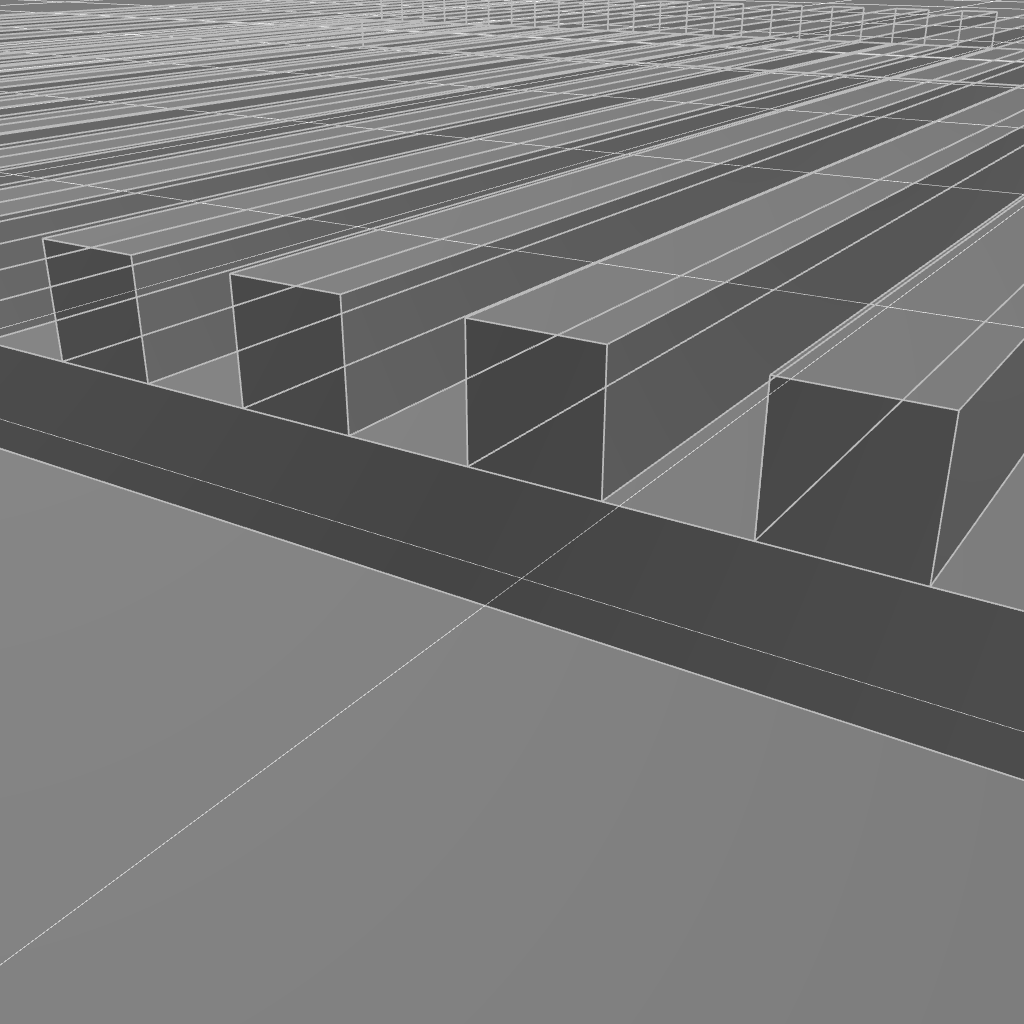
\includegraphics[width=0.9\linewidth]{img/diffusorNorm.png}
  \caption{\it Diffusor shape}
  \label{fig:diffNorm}
\end{subfigure}%
\begin{subfigure}[t]{0.2\textwidth}
  \centering
  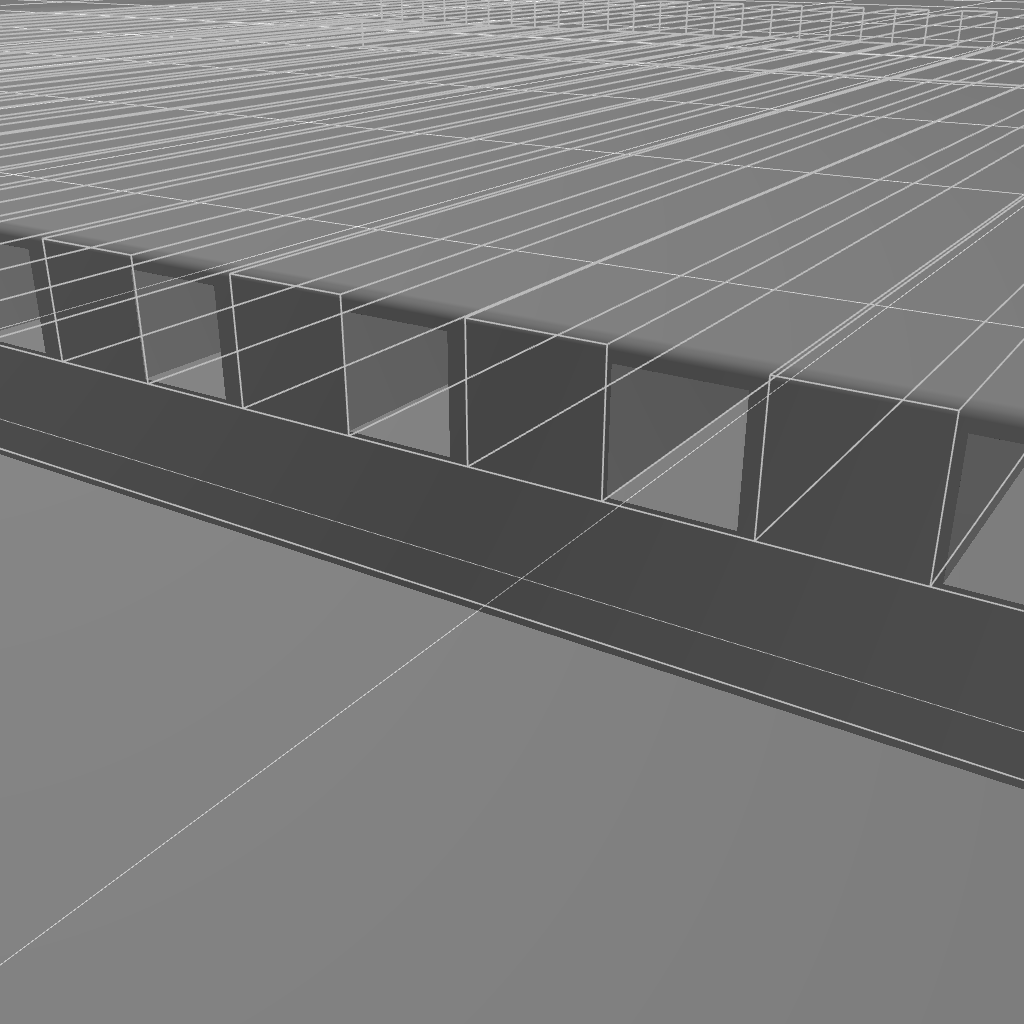
\includegraphics[width=0.9\linewidth]{img/diffusorSmooth.png}
  \caption{\it After subtraction: rounded and closed.}
  \label{fig:sub2}
\end{subfigure}
\caption{\it The diffusor from scene 1 in \cite{brinkmann_round_2019} was reconstructed exactly(a). A subtraction of $0.01$ from the distance function causes the holes to close(b).}
\label{fig:diffSmooth}
\end{figure}



% \begin{figure}[ht]
% \begin{subfigure}
% \centerline{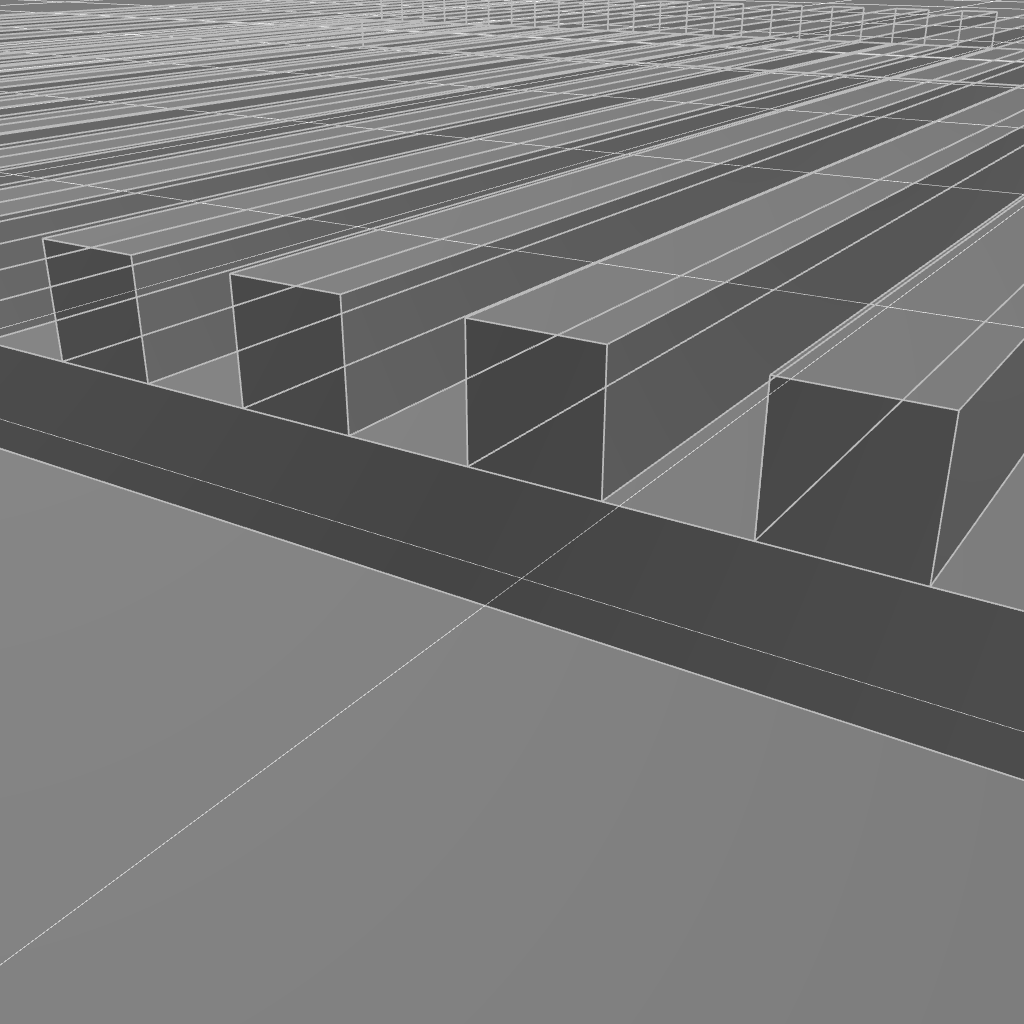
\includegraphics[scale=0.2]{img/diffusorNorm.png}}
% \caption{\label{diffusorSmoothing}{\it The diffusor from scene 1 in \cite{brinkmann_round_2019} was reconstructed exactly. A subtraction of $0.01$ from the distance function causes the holes to close.}}
% \end{subfigure}%
% \begin{subfigure}
% \centerline{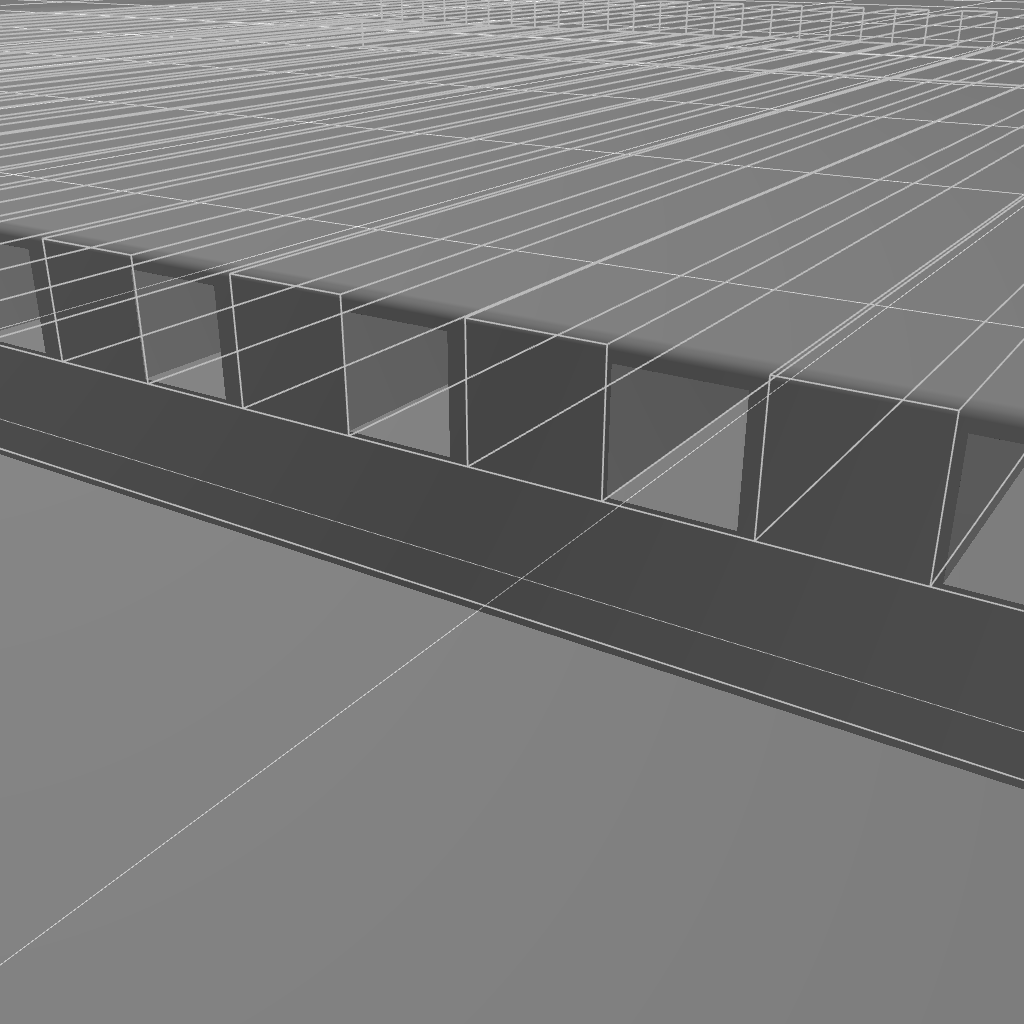
\includegraphics[scale=0.2]{img/diffusorSmooth.png}}
% \caption{\label{diffusorSmoothing}{\it The diffusor from scene 1 in \cite{brinkmann_round_2019} was reconstructed exactly. A subtraction of $0.01$ from the distance function causes the holes to close.}}
% \end{subfigure}

% \end{figure}  




procedural by default
deforming geometry
\subsubsection{Implementation}
It is possible to implement the chosen algorithm on the CPU and the GPU. A number of frameworks could be chosen for GPU accelerated computation such as OpenCL or NVIDIA CUDA. The choice of a shader has the advantage of being more operating system independent and hardware independent. Compute shaders (in contrast to fragment shaders) make it possible to write to arbitrary output locations which is necessary for generating the actual impulse response from the measurement of timings. Since they are available since OpenGL 4.3 (August 2012) / OpenGL ES 3.1 they are both aged enough to have received broad support in other frameworks and relatively new in respect to first publications about sphere tracing. Another reason for the choice of compute shaders is their simplicity. In comparison to CUDA and OpenCL, shaders are easier to write and the GLSL(Graphics Library Shading Language) is more widespread. Achieving the whole computation, from the definition of the geometry, to the ray tracing up until the actual impulse response computation in a single shader makes this attempt highly portable and expandable.


\section{Generation of SDFs}

Only rather simplistic shapes where needed for this proof-of-concept. Mostly boxes are used and combined in various ways to achieve reflection areas, shoe-box scenes and the little more complex diffusor shape of scene 1 in \cite{brinkmann_round_2019}. A simple 3D box SDF with a size of $R_x$x$R_y$x$R_z$ can be described by:

\begin{equation}
  f(p_x, p_y, p_z) = \sqrt{c_0(p_x - R_x)^2 + c_0(p_y - R_y)^2 + c_0(p_z - R_z)^2}
\end{equation}

where $c_0$ is just clipping at 0:

\begin{equation}
c_0(x) = max(x,0) 
\end{equation}

which translates to GLSL conveniently:

\begin{lstlisting}[language=C, caption={\it GLSL code for creating a box SDF},captionpos=b, label=lst:boxSdf]
float box(vec3 pos, vec3 R){
    return length(max(abs(pos) - R,0));
}
\end{lstlisting}

\cite{hart_sphere_1996} gives a list mathematical definitions of many shapes and for example \href{http://mercury.sexy/hg_sdf/}{http://mercury.sexy/hg\_sdf/} provides a rich and advanced library of shapes and operators that are ready to use for creation of more complex scenery.


\section{Sphere Tracing}
For simplicity, deterministic equal-angle Ray Tracing is used in contrast to Monte Carlo or Equal Area Ray tracing (EART) \cite{gu_room_2014}. Unidirectional ray tracing has been used, also for simplicity reasons, although \cite{cao_interactive_2016} has shown that bidirectional ray tracing offers advantages. Since the classical sphere tracing algorithm was adapted, it was found to be simplest to consider the "camera" to be the receiver/microphone as it would receive light. It sends out rays that might hit the sound source, which acts as a receiver of rays. The sound source is chosen to be a sphere. Choosing a correct volume for the receiver is critical and using a constant size can introduce systematic errors \cite{xiangyang_accuracy_2003}, \cite{alpkocak_computing_2010}. A number of models are available to compute the receiver Volume, $V_r$. Typically factors such as room volume, number of rays and the distance from source are used for this computation. 
As in \cite{brandao_ray_nodate}, \cite{alpkocak_computing_2010}, and \cite{dalenback_room_1996} the receiver was allowed to grow in volume. While \cite{brandao_ray_nodate} and \cite{dalenback_room_1996} use time to as a factor to let the receiver grow, in this attempt the reflection count, $k$ is used. Initially when a ray is sent, $k=1$ and when it hits a surface, this counter is increased by one so the source grows by this factor. Instead of using time, the model provided in \cite{alpkocak_computing_2010} is used and augmented with the $k$ term:
\begin{equation}
V_r = k \omega d_{SR}\sqrt{\frac{4}{N}}
\end{equation}
with 
\begin{equation}
\omega = log_{10}{V_{room}}
\end{equation}
where $d_{SR}$ is the source-receiver distance, $N$ is the number of initial rays and $V_{room}$ is the volume of the room.
The actual sphere tracing follows the original formulation in \cite{hart_sphere_1996}:

\begin{equation}
t_{i+1} = t_i + F(t_i)
\end{equation}
Here, this is implemented in the following way:
\begin{lstlisting}[language=C, caption={\it GLSL pseudo code for sphere tracing},captionpos=b,label=lst:sphereTrace]
for (i=0;i++;i<imax){
  vec3 pos = ro + t*rd;
  Sdf res = map(pos);
  t += res.x;
  if(res.x<epsilon){
    break
  }
}
\end{lstlisting} 

In the above simplified code listing, \texttt{ro} is a \texttt{vec3} that defines the ray origin, \texttt{rd} the ray direction and \texttt{epsilon} can be set to adjust the algorithms precision. The \texttt{map()} function in this case not only returns the distance computed via the SDF(\texttt{res.x}) but a \texttt{struct} that can contain material properties (reflection coefficients etc.). Here it was used to distinguish between a sound source and a regular reflective body.
The space is sampled spherically and \texttt{rd} is generated from the compute shader's \texttt{gl\_GlobalInvocationID}.
From there, the space is sampled using the following very simplified pseudo code:
\begin{lstlisting}[language=C, caption={\it GLSL pseudo code for sampling the space and writing to the RIR.},captionpos=b, label=lst:mainloop]
Sdf res = castRay(ro,rd)
for (int k=0;k<numReflections;k++;){
  if(ComingFromReflectiveBdy){
    rd = relect(rd,normal);
  }
  res = castRay(ro,rd);
  t = res.x;
  pos = ro+rd*t;
  if(res.body == soundSource){
    travelDistance+=t;
    readWrite(travelDistance,k);
  }
}

\end{lstlisting}

Here, \texttt{castRay()} refers to a function that looks similar to the sphere tracing function above and \texttt{readWrite()} refers to a function that takes the total distance a ray has travelled from source to receiver including all reflections and the number of reflections. From the distance it computes the location where to write to in the impulse response and the attenuation. It then reads the current value at this location and adds the corresponding value, making use of a compute shader's capability to read and write it's output and write to arbitrary output locations. The necessity to write to arbitrary output locations is the main reason for choosing a compute shader over a fragment shader. But it is possible to define most of the functionality to in one file that is included to a compute shader to calculate the RIR and to a fragment shader for visualization. This is particularly handy during construction of geometry.


\begin{figure}[ht]
\center
\begin{tikzpicture}

\node (lib) at (0,0) [rectangle,draw] {$F(p_{xyz})$};
\node (frag) at (-2,-1) [rectangle,draw] {$fragment\ shader$};
\node (comp) at (2,-1) [rectangle,draw] {$compute\ shader$};
\draw node [block, below of=frag, node distance = 1.5cm](rend){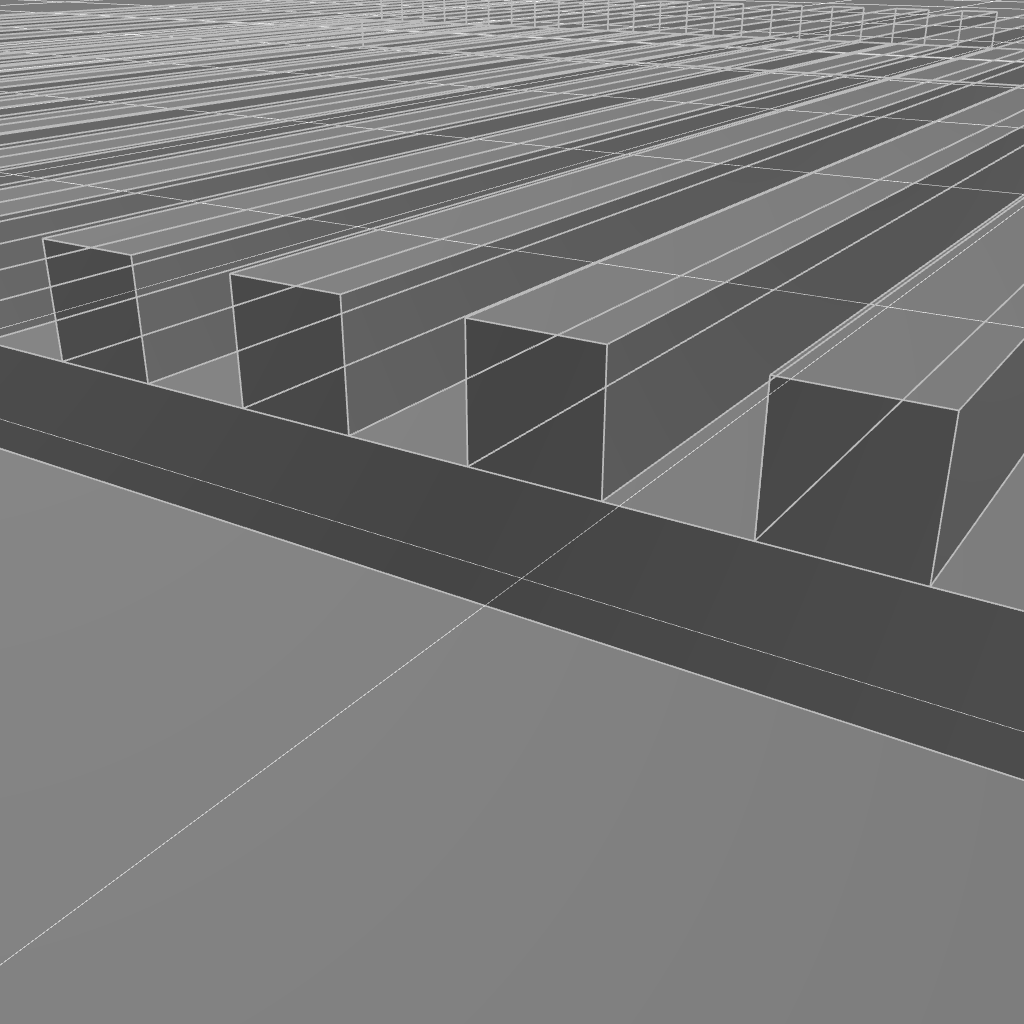
\includegraphics[width=.1\textwidth]{img/diffusorNorm.png}};
\draw node [block, below of=comp, node distance = 1.5cm](H){$H(n)$};
% \node (rend) [rectangle,draw, below=frag] {$compute\ shader$};
\draw[->] (lib) -- node {} (frag);
\draw[->] (lib) -- node {} (comp);
\draw[->] (frag) -- node {}(rend);
\draw[->] (comp) -- node {}(H);

% \draw[->,thick] (lib) to (comp);
% \draw[->,thick] (lib) to (comp);


\end{tikzpicture}
\caption{\label{fig:bd_shaders}{\it A lot of the code, especially the map function, $F(p_{xyz})$, which contains the SDF can be shared between a fragment shader used for visualization and a compute shader responsible for RIR calculation.}}
\end{figure}



\begin{enumerate}
\item reflection
\item low frequency pass
\end{enumerate}


\section{Generation of impulse response}
The room is assumed to a linear time invariant system(LTI). Due to the proof-of-concept nature of this proposal, a highly simplified model for RIR computation is used. Sphere tracing delivers distances and number of reflections for $M$ rays in this implementation. Each ray follows a number of reflections $K(m)$. Each reflection pass adds up to a total travel distance of the ray, $d(m)$. The sound source is assumed to send out a discrete impulse, the kronecker delta function, $\delta(n)$. As non-integer delays are ignored in this implementation, the shader will just write to the rounded integer delay location $\tau_s$ in the impulse response, $H(n)$,that corresponds to the distance:
\begin{equation}
H(n) = \sum_{m=0}^M \delta(n-\tau_s(m))\cdot \alpha(m)\cdot -1^{K(m)}
\end{equation}
The total attenuation per ray $\alpha(m)$ can be computed by using a material dependent coefficient of reflection $\alpha_{mat}$ that is stored in the \texttt{Sdf struct}. At each reflection pass $k$ this results in a possibly different reflection pass dependent coefficient $\alpha_{mat}(k,m)$ and keeping a running product in the loop of Listing \ref{lst:mainloop}:
\begin{equation}
\alpha(m)=\prod_{k=0}^{K(m)} \alpha_{mat}(k,m)
\end{equation}
For simplicity's sake, here only one global coefficient $\alpha_G$ is implemented resulting in:
\begin{equation}
\alpha(m) = \alpha_G^{K(m)}
\end{equation}

Additionally, a proof-of-concept for frequency dependent loss for each reflection is introduced into the model. As a computationally efficient heuristic, a simple one-zero filter $G(z)$ is applied at each reflection:

\begin{equation}
G(z,K) = (1+z^{-1})^K \cdot \frac{1}{2}^K
\end{equation}
The advantage of using such a simple filter is that a $K$-stage cascade's impulse response can be computed easily without applying the filter repeatedly. By doing the discrete time inverse fourier transform of the transfer function $Gz$ the $N$-length impulse response is obtained:

\begin{equation}
  G(n,K) = \mathfrak{F}^{-1}\{ G(z) \} = (\frac{1}{2})^K \frac{1}{N}  \sum_{\omega = 0}^\pi (1+e^{-j\omega})^{K} e^{j\omega n} 
\end{equation}

Numerically, it can easily be shown that

\begin{equation}
G(n,K) \approx  \frac{1}{\sigma \cdot \sqrt{2 \pi}} \cdot e ^{-\frac{1}{2} (\frac{n-\mu}{\sigma})^2}
\label{eq:assump}
\end{equation}


with 

\begin{equation}
\sigma \approx \sqrt{K 0.231 + 0.562}
\end{equation}

\begin{equation}
\mu \approx \frac{K}{2} + \frac{1}{2}
\end{equation}

The right hand side of Equation \ref{eq:assump} is simply the normal distribution, which is computationally efficient to calculate for any $K$.

So instead of adding $\delta(n-\tau(m))$ into the IR, simply $G(n-\tau(m),K)$ is used. Similar to many other implementations, a high-pass filter is applied to the resulting RIR.




\begin{figure}
    \begin{center}
      % This file was created by tikzplotlib v0.9.1.
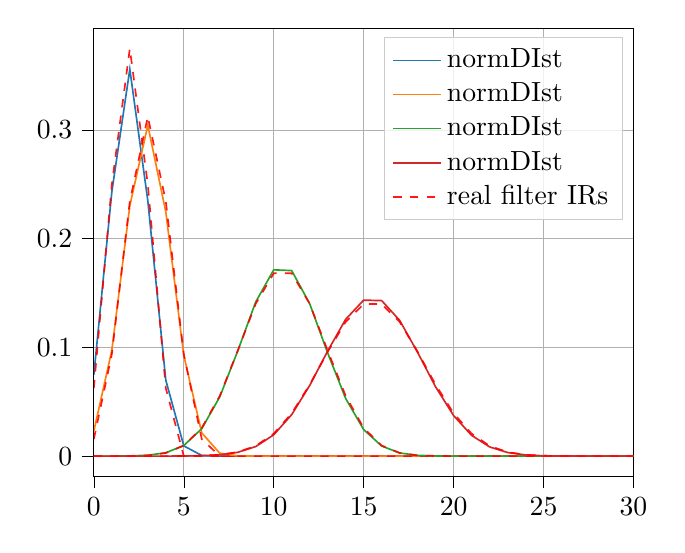
\begin{tikzpicture}

\definecolor{color0}{rgb}{0.1216,0.4667,0.7059}
\definecolor{color1}{rgb}{1.0000,0.4980,0.0549}
\definecolor{color2}{rgb}{0.1725,0.6275,0.1725}
\definecolor{color3}{rgb}{0.8392,0.1529,0.1569}

\begin{axis}[
legend cell align={left},
legend style={fill opacity=0.8, draw opacity=1, text opacity=1, draw=white!80.0000!black},
tick align=outside,
tick pos=left,
x grid style={white!69.0196!black},
xmajorgrids,
xmin=0.0000, xmax=30.0000,
xtick style={color=black},
y grid style={white!69.0196!black},
ymajorgrids,
ymin=-0.0188, ymax=0.3937,
ytick style={color=black}
]
\addplot [semithick, color0]
table {%
0.0000 0.0749
1.0000 0.2432
2.0000 0.3560
3.0000 0.2350
4.0000 0.0699
5.0000 0.0094
6.0000 0.0006
7.0000 0.0000
8.0000 0.0000
9.0000 0.0000
10.0000 0.0000
11.0000 0.0000
12.0000 0.0000
13.0000 0.0000
14.0000 0.0000
15.0000 0.0000
16.0000 0.0000
17.0000 0.0000
18.0000 0.0000
19.0000 0.0000
20.0000 0.0000
21.0000 0.0000
22.0000 0.0000
23.0000 0.0000
24.0000 0.0000
25.0000 0.0000
26.0000 0.0000
27.0000 0.0000
28.0000 0.0000
29.0000 0.0000
30.0000 0.0000
31.0000 0.0000
32.0000 0.0000
33.0000 0.0000
34.0000 0.0000
35.0000 0.0000
36.0000 0.0000
37.0000 0.0000
38.0000 0.0000
39.0000 0.0000
40.0000 0.0000
41.0000 0.0000
42.0000 0.0000
43.0000 0.0000
44.0000 0.0000
45.0000 0.0000
46.0000 0.0000
47.0000 0.0000
48.0000 0.0000
49.0000 0.0000
50.0000 0.0000
51.0000 0.0000
52.0000 0.0000
53.0000 0.0000
54.0000 0.0000
55.0000 0.0000
56.0000 0.0000
57.0000 0.0000
58.0000 0.0000
59.0000 0.0000
60.0000 0.0000
61.0000 0.0000
62.0000 0.0000
63.0000 0.0000
64.0000 0.0000
65.0000 0.0000
66.0000 0.0000
67.0000 0.0000
68.0000 0.0000
69.0000 0.0000
70.0000 0.0000
71.0000 0.0000
72.0000 0.0000
73.0000 0.0000
74.0000 0.0000
75.0000 0.0000
76.0000 0.0000
77.0000 0.0000
78.0000 0.0000
79.0000 0.0000
80.0000 0.0000
81.0000 0.0000
82.0000 0.0000
83.0000 0.0000
84.0000 0.0000
85.0000 0.0000
86.0000 0.0000
87.0000 0.0000
88.0000 0.0000
89.0000 0.0000
90.0000 0.0000
91.0000 0.0000
92.0000 0.0000
93.0000 0.0000
94.0000 0.0000
95.0000 0.0000
96.0000 0.0000
97.0000 0.0000
98.0000 0.0000
99.0000 0.0000
};
\addlegendentry{normDIst}
\addplot [semithick, red, opacity=0.9, dashed, forget plot]
table {%
0.0000 0.0625
1.0000 0.2500
2.0000 0.3750
3.0000 0.2500
4.0000 0.0625
5.0000 0.0000
6.0000 0.0000
7.0000 0.0000
8.0000 0.0000
9.0000 0.0000
10.0000 0.0000
11.0000 0.0000
12.0000 0.0000
13.0000 0.0000
14.0000 0.0000
15.0000 0.0000
16.0000 0.0000
17.0000 0.0000
18.0000 0.0000
19.0000 0.0000
20.0000 0.0000
21.0000 0.0000
22.0000 0.0000
23.0000 0.0000
24.0000 0.0000
25.0000 0.0000
26.0000 0.0000
27.0000 0.0000
28.0000 0.0000
29.0000 0.0000
30.0000 0.0000
31.0000 0.0000
32.0000 0.0000
33.0000 0.0000
34.0000 0.0000
35.0000 0.0000
36.0000 0.0000
37.0000 0.0000
38.0000 0.0000
39.0000 0.0000
40.0000 0.0000
41.0000 0.0000
42.0000 0.0000
43.0000 0.0000
44.0000 0.0000
45.0000 0.0000
46.0000 0.0000
47.0000 0.0000
48.0000 0.0000
49.0000 0.0000
50.0000 0.0000
51.0000 0.0000
52.0000 0.0000
53.0000 0.0000
54.0000 0.0000
55.0000 0.0000
56.0000 0.0000
57.0000 0.0000
58.0000 0.0000
59.0000 0.0000
60.0000 0.0000
61.0000 0.0000
62.0000 0.0000
63.0000 0.0000
64.0000 0.0000
65.0000 0.0000
66.0000 0.0000
67.0000 0.0000
68.0000 0.0000
69.0000 0.0000
70.0000 0.0000
71.0000 0.0000
72.0000 0.0000
73.0000 0.0000
74.0000 0.0000
75.0000 0.0000
76.0000 0.0000
77.0000 0.0000
78.0000 0.0000
79.0000 0.0000
80.0000 0.0000
81.0000 0.0000
82.0000 0.0000
83.0000 0.0000
84.0000 0.0000
85.0000 0.0000
86.0000 0.0000
87.0000 0.0000
88.0000 0.0000
89.0000 0.0000
90.0000 0.0000
91.0000 0.0000
92.0000 0.0000
93.0000 0.0000
94.0000 0.0000
95.0000 0.0000
96.0000 0.0000
97.0000 0.0000
98.0000 0.0000
99.0000 0.0000
};
\addplot [semithick, color1]
table {%
0.0000 0.0230
1.0000 0.0974
2.0000 0.2304
3.0000 0.3044
4.0000 0.2247
5.0000 0.0926
6.0000 0.0213
7.0000 0.0027
8.0000 0.0002
9.0000 0.0000
10.0000 0.0000
11.0000 0.0000
12.0000 0.0000
13.0000 0.0000
14.0000 0.0000
15.0000 0.0000
16.0000 0.0000
17.0000 0.0000
18.0000 0.0000
19.0000 0.0000
20.0000 0.0000
21.0000 0.0000
22.0000 0.0000
23.0000 0.0000
24.0000 0.0000
25.0000 0.0000
26.0000 0.0000
27.0000 0.0000
28.0000 0.0000
29.0000 0.0000
30.0000 0.0000
31.0000 0.0000
32.0000 0.0000
33.0000 0.0000
34.0000 0.0000
35.0000 0.0000
36.0000 0.0000
37.0000 0.0000
38.0000 0.0000
39.0000 0.0000
40.0000 0.0000
41.0000 0.0000
42.0000 0.0000
43.0000 0.0000
44.0000 0.0000
45.0000 0.0000
46.0000 0.0000
47.0000 0.0000
48.0000 0.0000
49.0000 0.0000
50.0000 0.0000
51.0000 0.0000
52.0000 0.0000
53.0000 0.0000
54.0000 0.0000
55.0000 0.0000
56.0000 0.0000
57.0000 0.0000
58.0000 0.0000
59.0000 0.0000
60.0000 0.0000
61.0000 0.0000
62.0000 0.0000
63.0000 0.0000
64.0000 0.0000
65.0000 0.0000
66.0000 0.0000
67.0000 0.0000
68.0000 0.0000
69.0000 0.0000
70.0000 0.0000
71.0000 0.0000
72.0000 0.0000
73.0000 0.0000
74.0000 0.0000
75.0000 0.0000
76.0000 0.0000
77.0000 0.0000
78.0000 0.0000
79.0000 0.0000
80.0000 0.0000
81.0000 0.0000
82.0000 0.0000
83.0000 0.0000
84.0000 0.0000
85.0000 0.0000
86.0000 0.0000
87.0000 0.0000
88.0000 0.0000
89.0000 0.0000
90.0000 0.0000
91.0000 0.0000
92.0000 0.0000
93.0000 0.0000
94.0000 0.0000
95.0000 0.0000
96.0000 0.0000
97.0000 0.0000
98.0000 0.0000
99.0000 0.0000
};
\addlegendentry{normDIst}
\addplot [semithick, red, opacity=0.9, dashed, forget plot]
table {%
0.0000 0.0156
1.0000 0.0938
2.0000 0.2344
3.0000 0.3125
4.0000 0.2344
5.0000 0.0938
6.0000 0.0156
7.0000 0.0000
8.0000 0.0000
9.0000 0.0000
10.0000 0.0000
11.0000 0.0000
12.0000 0.0000
13.0000 0.0000
14.0000 0.0000
15.0000 0.0000
16.0000 0.0000
17.0000 0.0000
18.0000 0.0000
19.0000 0.0000
20.0000 0.0000
21.0000 0.0000
22.0000 0.0000
23.0000 0.0000
24.0000 0.0000
25.0000 0.0000
26.0000 0.0000
27.0000 0.0000
28.0000 0.0000
29.0000 0.0000
30.0000 0.0000
31.0000 0.0000
32.0000 0.0000
33.0000 0.0000
34.0000 0.0000
35.0000 0.0000
36.0000 0.0000
37.0000 0.0000
38.0000 0.0000
39.0000 0.0000
40.0000 0.0000
41.0000 0.0000
42.0000 0.0000
43.0000 0.0000
44.0000 0.0000
45.0000 0.0000
46.0000 0.0000
47.0000 0.0000
48.0000 0.0000
49.0000 0.0000
50.0000 0.0000
51.0000 0.0000
52.0000 0.0000
53.0000 0.0000
54.0000 0.0000
55.0000 0.0000
56.0000 0.0000
57.0000 0.0000
58.0000 0.0000
59.0000 0.0000
60.0000 0.0000
61.0000 0.0000
62.0000 0.0000
63.0000 0.0000
64.0000 0.0000
65.0000 0.0000
66.0000 0.0000
67.0000 0.0000
68.0000 0.0000
69.0000 0.0000
70.0000 0.0000
71.0000 0.0000
72.0000 0.0000
73.0000 0.0000
74.0000 0.0000
75.0000 0.0000
76.0000 0.0000
77.0000 0.0000
78.0000 0.0000
79.0000 0.0000
80.0000 0.0000
81.0000 0.0000
82.0000 0.0000
83.0000 0.0000
84.0000 0.0000
85.0000 0.0000
86.0000 0.0000
87.0000 0.0000
88.0000 0.0000
89.0000 0.0000
90.0000 0.0000
91.0000 0.0000
92.0000 0.0000
93.0000 0.0000
94.0000 0.0000
95.0000 0.0000
96.0000 0.0000
97.0000 0.0000
98.0000 0.0000
99.0000 0.0000
};
\addplot [semithick, color2]
table {%
0.0000 0.0000
1.0000 0.0000
2.0000 0.0002
3.0000 0.0008
4.0000 0.0031
5.0000 0.0097
6.0000 0.0253
7.0000 0.0545
8.0000 0.0968
9.0000 0.1419
10.0000 0.1714
11.0000 0.1707
12.0000 0.1402
13.0000 0.0949
14.0000 0.0530
15.0000 0.0244
16.0000 0.0093
17.0000 0.0029
18.0000 0.0007
19.0000 0.0002
20.0000 0.0000
21.0000 0.0000
22.0000 0.0000
23.0000 0.0000
24.0000 0.0000
25.0000 0.0000
26.0000 0.0000
27.0000 0.0000
28.0000 0.0000
29.0000 0.0000
30.0000 0.0000
31.0000 0.0000
32.0000 0.0000
33.0000 0.0000
34.0000 0.0000
35.0000 0.0000
36.0000 0.0000
37.0000 0.0000
38.0000 0.0000
39.0000 0.0000
40.0000 0.0000
41.0000 0.0000
42.0000 0.0000
43.0000 0.0000
44.0000 0.0000
45.0000 0.0000
46.0000 0.0000
47.0000 0.0000
48.0000 0.0000
49.0000 0.0000
50.0000 0.0000
51.0000 0.0000
52.0000 0.0000
53.0000 0.0000
54.0000 0.0000
55.0000 0.0000
56.0000 0.0000
57.0000 0.0000
58.0000 0.0000
59.0000 0.0000
60.0000 0.0000
61.0000 0.0000
62.0000 0.0000
63.0000 0.0000
64.0000 0.0000
65.0000 0.0000
66.0000 0.0000
67.0000 0.0000
68.0000 0.0000
69.0000 0.0000
70.0000 0.0000
71.0000 0.0000
72.0000 0.0000
73.0000 0.0000
74.0000 0.0000
75.0000 0.0000
76.0000 0.0000
77.0000 0.0000
78.0000 0.0000
79.0000 0.0000
80.0000 0.0000
81.0000 0.0000
82.0000 0.0000
83.0000 0.0000
84.0000 0.0000
85.0000 0.0000
86.0000 0.0000
87.0000 0.0000
88.0000 0.0000
89.0000 0.0000
90.0000 0.0000
91.0000 0.0000
92.0000 0.0000
93.0000 0.0000
94.0000 0.0000
95.0000 0.0000
96.0000 0.0000
97.0000 0.0000
98.0000 0.0000
99.0000 0.0000
};
\addlegendentry{normDIst}
\addplot [semithick, red, opacity=0.9, dashed, forget plot]
table {%
0.0000 0.0000
1.0000 0.0000
2.0000 0.0001
3.0000 0.0006
4.0000 0.0029
5.0000 0.0097
6.0000 0.0259
7.0000 0.0554
8.0000 0.0970
9.0000 0.1402
10.0000 0.1682
11.0000 0.1682
12.0000 0.1402
13.0000 0.0970
14.0000 0.0554
15.0000 0.0259
16.0000 0.0097
17.0000 0.0029
18.0000 0.0006
19.0000 0.0001
20.0000 0.0000
21.0000 0.0000
22.0000 0.0000
23.0000 0.0000
24.0000 0.0000
25.0000 0.0000
26.0000 0.0000
27.0000 0.0000
28.0000 0.0000
29.0000 0.0000
30.0000 0.0000
31.0000 0.0000
32.0000 0.0000
33.0000 0.0000
34.0000 0.0000
35.0000 0.0000
36.0000 0.0000
37.0000 0.0000
38.0000 0.0000
39.0000 0.0000
40.0000 0.0000
41.0000 0.0000
42.0000 0.0000
43.0000 0.0000
44.0000 0.0000
45.0000 0.0000
46.0000 0.0000
47.0000 0.0000
48.0000 0.0000
49.0000 0.0000
50.0000 0.0000
51.0000 0.0000
52.0000 0.0000
53.0000 0.0000
54.0000 0.0000
55.0000 0.0000
56.0000 0.0000
57.0000 0.0000
58.0000 0.0000
59.0000 0.0000
60.0000 0.0000
61.0000 0.0000
62.0000 0.0000
63.0000 0.0000
64.0000 0.0000
65.0000 0.0000
66.0000 0.0000
67.0000 0.0000
68.0000 0.0000
69.0000 0.0000
70.0000 0.0000
71.0000 0.0000
72.0000 0.0000
73.0000 0.0000
74.0000 0.0000
75.0000 0.0000
76.0000 0.0000
77.0000 0.0000
78.0000 0.0000
79.0000 0.0000
80.0000 0.0000
81.0000 0.0000
82.0000 0.0000
83.0000 0.0000
84.0000 0.0000
85.0000 0.0000
86.0000 0.0000
87.0000 0.0000
88.0000 0.0000
89.0000 0.0000
90.0000 0.0000
91.0000 0.0000
92.0000 0.0000
93.0000 0.0000
94.0000 0.0000
95.0000 0.0000
96.0000 0.0000
97.0000 0.0000
98.0000 0.0000
99.0000 0.0000
};
\addplot [semithick, color3]
table {%
0.0000 0.0000
1.0000 0.0000
2.0000 0.0000
3.0000 0.0000
4.0000 0.0000
5.0000 0.0001
6.0000 0.0004
7.0000 0.0012
8.0000 0.0035
9.0000 0.0088
10.0000 0.0196
11.0000 0.0382
12.0000 0.0650
13.0000 0.0967
14.0000 0.1259
15.0000 0.1435
16.0000 0.1431
17.0000 0.1249
18.0000 0.0954
19.0000 0.0637
20.0000 0.0373
21.0000 0.0191
22.0000 0.0085
23.0000 0.0033
24.0000 0.0011
25.0000 0.0003
26.0000 0.0001
27.0000 0.0000
28.0000 0.0000
29.0000 0.0000
30.0000 0.0000
31.0000 0.0000
32.0000 0.0000
33.0000 0.0000
34.0000 0.0000
35.0000 0.0000
36.0000 0.0000
37.0000 0.0000
38.0000 0.0000
39.0000 0.0000
40.0000 0.0000
41.0000 0.0000
42.0000 0.0000
43.0000 0.0000
44.0000 0.0000
45.0000 0.0000
46.0000 0.0000
47.0000 0.0000
48.0000 0.0000
49.0000 0.0000
50.0000 0.0000
51.0000 0.0000
52.0000 0.0000
53.0000 0.0000
54.0000 0.0000
55.0000 0.0000
56.0000 0.0000
57.0000 0.0000
58.0000 0.0000
59.0000 0.0000
60.0000 0.0000
61.0000 0.0000
62.0000 0.0000
63.0000 0.0000
64.0000 0.0000
65.0000 0.0000
66.0000 0.0000
67.0000 0.0000
68.0000 0.0000
69.0000 0.0000
70.0000 0.0000
71.0000 0.0000
72.0000 0.0000
73.0000 0.0000
74.0000 0.0000
75.0000 0.0000
76.0000 0.0000
77.0000 0.0000
78.0000 0.0000
79.0000 0.0000
80.0000 0.0000
81.0000 0.0000
82.0000 0.0000
83.0000 0.0000
84.0000 0.0000
85.0000 0.0000
86.0000 0.0000
87.0000 0.0000
88.0000 0.0000
89.0000 0.0000
90.0000 0.0000
91.0000 0.0000
92.0000 0.0000
93.0000 0.0000
94.0000 0.0000
95.0000 0.0000
96.0000 0.0000
97.0000 0.0000
98.0000 0.0000
99.0000 0.0000
};
\addlegendentry{normDIst}
\addplot [semithick, red, opacity=0.9, dashed]
table {%
0.0000 0.0000
1.0000 0.0000
2.0000 0.0000
3.0000 0.0000
4.0000 0.0000
5.0000 0.0001
6.0000 0.0003
7.0000 0.0012
8.0000 0.0037
9.0000 0.0094
10.0000 0.0207
11.0000 0.0394
12.0000 0.0657
13.0000 0.0960
14.0000 0.1235
15.0000 0.1399
16.0000 0.1399
17.0000 0.1235
18.0000 0.0960
19.0000 0.0657
20.0000 0.0394
21.0000 0.0207
22.0000 0.0094
23.0000 0.0037
24.0000 0.0012
25.0000 0.0003
26.0000 0.0001
27.0000 0.0000
28.0000 0.0000
29.0000 0.0000
30.0000 0.0000
31.0000 0.0000
32.0000 0.0000
33.0000 0.0000
34.0000 0.0000
35.0000 0.0000
36.0000 0.0000
37.0000 0.0000
38.0000 0.0000
39.0000 0.0000
40.0000 0.0000
41.0000 0.0000
42.0000 0.0000
43.0000 0.0000
44.0000 0.0000
45.0000 0.0000
46.0000 0.0000
47.0000 0.0000
48.0000 0.0000
49.0000 0.0000
50.0000 0.0000
51.0000 0.0000
52.0000 0.0000
53.0000 0.0000
54.0000 0.0000
55.0000 0.0000
56.0000 0.0000
57.0000 0.0000
58.0000 0.0000
59.0000 0.0000
60.0000 0.0000
61.0000 0.0000
62.0000 0.0000
63.0000 0.0000
64.0000 0.0000
65.0000 0.0000
66.0000 0.0000
67.0000 0.0000
68.0000 0.0000
69.0000 0.0000
70.0000 0.0000
71.0000 0.0000
72.0000 0.0000
73.0000 0.0000
74.0000 0.0000
75.0000 0.0000
76.0000 0.0000
77.0000 0.0000
78.0000 0.0000
79.0000 0.0000
80.0000 0.0000
81.0000 0.0000
82.0000 0.0000
83.0000 0.0000
84.0000 0.0000
85.0000 0.0000
86.0000 0.0000
87.0000 0.0000
88.0000 0.0000
89.0000 0.0000
90.0000 0.0000
91.0000 0.0000
92.0000 0.0000
93.0000 0.0000
94.0000 0.0000
95.0000 0.0000
96.0000 0.0000
97.0000 0.0000
98.0000 0.0000
99.0000 0.0000
};
\addlegendentry{real filter IRs}
\end{axis}

\end{tikzpicture}

        % % This file was created by tikzplotlib v0.9.1.
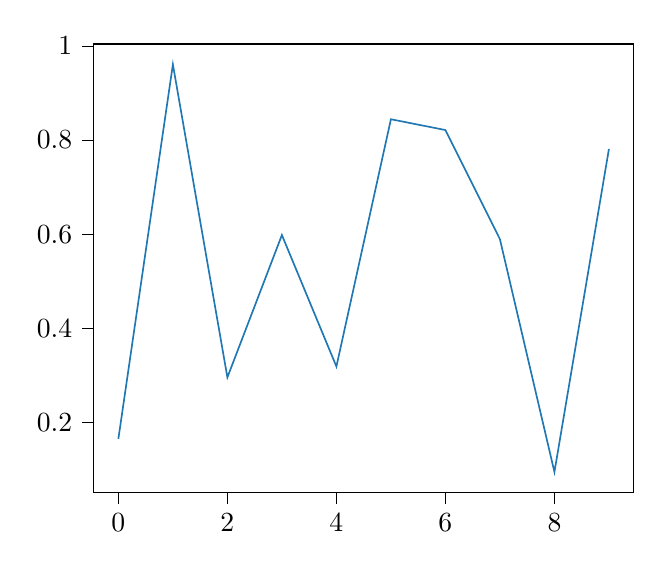
\begin{tikzpicture}

\definecolor{color0}{rgb}{0.12156862745098,0.466666666666667,0.705882352941177}

\begin{axis}[
tick align=outside,
tick pos=left,
x grid style={white!69.0196078431373!black},
xmin=-0.45, xmax=9.45,
xtick style={color=black},
y grid style={white!69.0196078431373!black},
ymin=0.0515297644926165, ymax=1.0037743262763,
ytick style={color=black}
]
\addplot [semithick, color0]
table {%
0 0.165204368712852
1 0.960490482558861
2 0.295706783168825
3 0.598084081751131
4 0.318814100655487
5 0.844017623549353
6 0.821076195130074
7 0.589191813076777
8 0.0948136082100567
9 0.781036863745426
};
\end{axis}

\end{tikzpicture}

    \end{center}
    \caption{A PGF histogram from \texttt{matplotlib}.}
\end{figure}


% Advantage of compute shader.
% Maybe introduce cascaded Lowpass.



% All figures should be centred on the column (or page, if the figure spans both columns).
% Figure captions (in italic) should follow each figure and have the format given in Figure \ref{fft_plot}.
% %
% Vectorial figures are preferred. For example when using
% \texttt{Matlab}, export using either Postscript or PDF format. Also,
% in order to provide a better readability, figure text font size
% should be at least identical to footnote font size. To do so using
% \texttt{Matlab}, use the \texttt{subplot} command before plotting.
% If bitmap figures are used, please make sure that the resolution is
% enough for print quality. Fig. \ref{ftt_plot2} illustrates an
% example of a figure spanning two columns.
%

\section{Results}
\begin{enumerate}
\item compare to \cite{brinkmann_round_2019}
\item compare to \cite{campbell_roomsim_nodate}
\end{enumerate}


% \begin{figure}[ht]
% \centerline{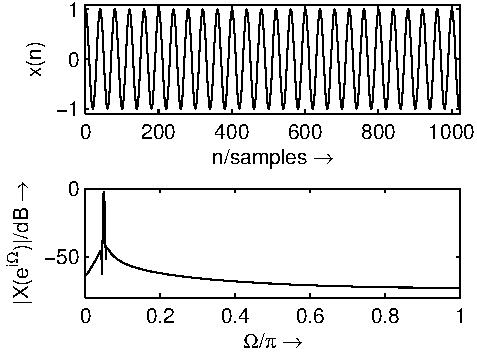
\includegraphics[scale=0.8]{fft_plot2}}
% \caption{\label{fft_plot}{\it Sinusoid in time and frequency domain. Short captions are centred, long captions (more than 1 line) are justified.}}
% \end{figure}
% %
% \begin{figure*}[ht]
% \center
% 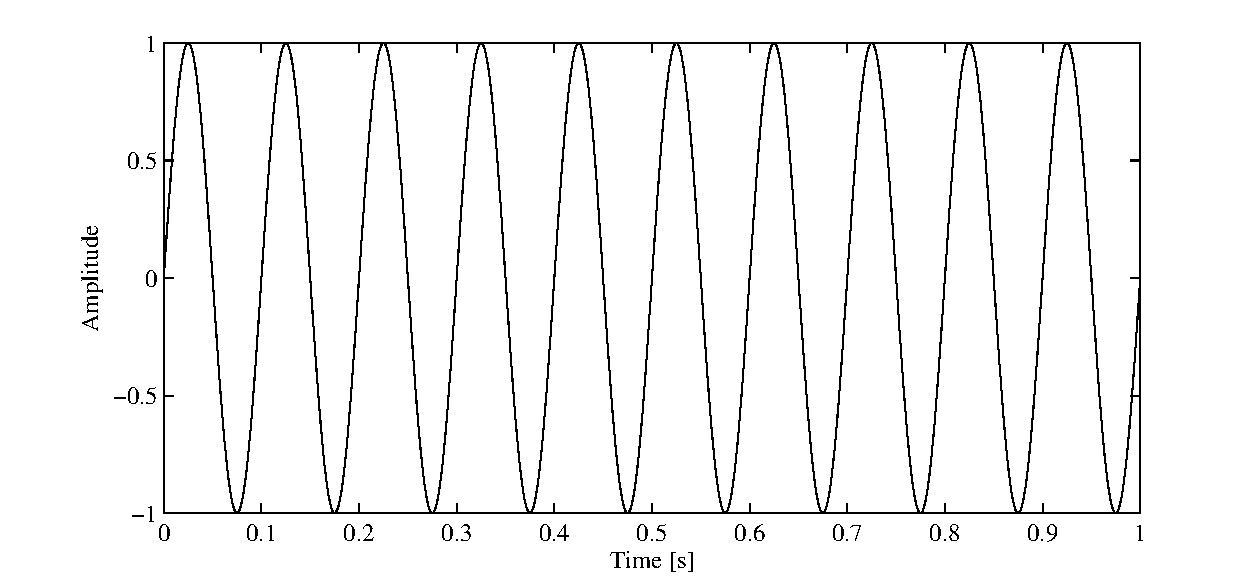
\includegraphics[width=5in]{TwoColumnSine2}
% \caption{\label{ftt_plot2}{\it A figure spanning two columns, as mentioned in Sec. . }}
% \end{figure*}


% \begin{figure}[ht]
% \centerline{\includegraphics[scale=0.8]{img/test1.pgf}}
% \caption{\label{fft_plot}{\it Sinusoid in time and frequency domain. Short captions are centred, long captions (more than 1 line) are justified.}}
% \end{figure}

\begin{figure}
    \begin{center}
      % This file was created by tikzplotlib v0.9.1.
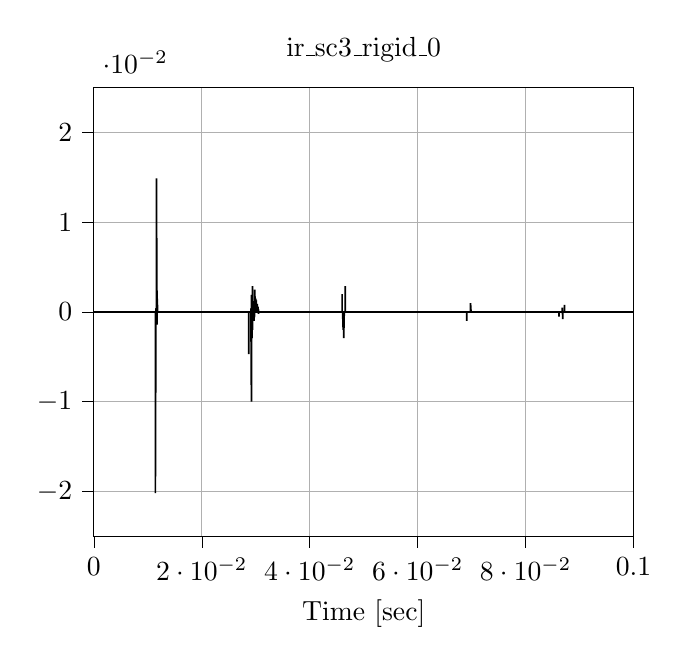
\begin{tikzpicture}

\begin{axis}[
tick align=outside,
tick pos=left,
title={ir\_sc3\_rigid\_0},
x grid style={white!69.0196!black},
xlabel={Time [sec]},
xmajorgrids,
xmin=0.0000, xmax=0.1000,
xtick style={color=black},
y grid style={white!69.0196!black},
ymajorgrids,
ymin=-0.0250, ymax=0.0250,
ytick style={color=black}
]
\addplot [semithick, black]
table {%
0.0000 0.0000
0.0114 0.0000
0.0114 -0.0202
0.0115 0.0000
0.0115 0.0000
0.0115 0.0000
0.0115 0.0001
0.0116 0.0000
0.0116 0.0001
0.0116 0.0149
0.0117 -0.0014
0.0117 0.0024
0.0117 0.0003
0.0117 0.0020
0.0118 0.0005
0.0118 0.0000
0.0121 0.0000
0.0287 0.0000
0.0287 -0.0047
0.0287 0.0000
0.0291 0.0000
0.0291 0.0004
0.0292 -0.0100
0.0292 0.0019
0.0292 -0.0009
0.0292 -0.0006
0.0293 0.0004
0.0293 -0.0001
0.0293 -0.0000
0.0293 0.0004
0.0293 -0.0029
0.0294 0.0029
0.0294 -0.0020
0.0294 0.0018
0.0295 -0.0001
0.0295 0.0000
0.0295 0.0009
0.0295 -0.0009
0.0295 0.0012
0.0296 -0.0004
0.0296 0.0000
0.0296 -0.0005
0.0297 0.0010
0.0297 -0.0010
0.0297 0.0011
0.0297 -0.0008
0.0298 0.0013
0.0298 -0.0005
0.0298 0.0025
0.0299 0.0009
0.0299 0.0012
0.0299 0.0007
0.0300 0.0011
0.0300 0.0007
0.0300 -0.0001
0.0300 0.0015
0.0300 0.0005
0.0301 0.0007
0.0301 0.0004
0.0301 0.0008
0.0302 0.0004
0.0302 0.0008
0.0302 0.0002
0.0302 0.0007
0.0303 0.0006
0.0303 -0.0001
0.0303 0.0009
0.0303 -0.0000
0.0304 0.0006
0.0304 0.0004
0.0304 0.0000
0.0304 0.0006
0.0305 -0.0002
0.0305 0.0003
0.0305 0.0000
0.0460 0.0000
0.0460 0.0020
0.0460 -0.0000
0.0461 -0.0000
0.0462 -0.0020
0.0462 0.0000
0.0463 0.0000
0.0463 -0.0029
0.0464 -0.0000
0.0465 0.0000
0.0466 0.0000
0.0466 0.0029
0.0466 0.0000
0.0691 0.0000
0.0691 -0.0010
0.0691 0.0000
0.0698 0.0000
0.0698 0.0010
0.0699 0.0000
0.0862 0.0000
0.0862 -0.0005
0.0862 0.0000
0.0868 0.0000
0.0868 0.0005
0.0869 -0.0008
0.0869 0.0000
0.0872 0.0000
0.0872 0.0008
0.0872 0.0000
0.1000 0.0000
};
\end{axis}

\end{tikzpicture}

        % % This file was created by tikzplotlib v0.9.1.
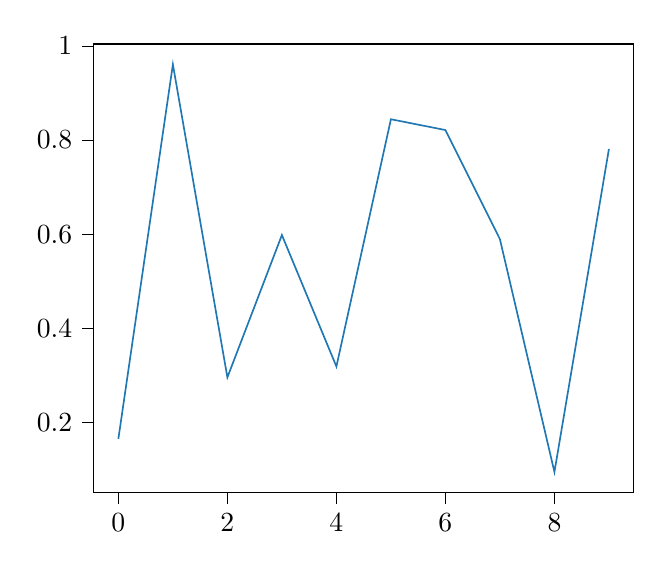
\begin{tikzpicture}

\definecolor{color0}{rgb}{0.12156862745098,0.466666666666667,0.705882352941177}

\begin{axis}[
tick align=outside,
tick pos=left,
x grid style={white!69.0196078431373!black},
xmin=-0.45, xmax=9.45,
xtick style={color=black},
y grid style={white!69.0196078431373!black},
ymin=0.0515297644926165, ymax=1.0037743262763,
ytick style={color=black}
]
\addplot [semithick, color0]
table {%
0 0.165204368712852
1 0.960490482558861
2 0.295706783168825
3 0.598084081751131
4 0.318814100655487
5 0.844017623549353
6 0.821076195130074
7 0.589191813076777
8 0.0948136082100567
9 0.781036863745426
};
\end{axis}

\end{tikzpicture}

    \end{center}
    \caption{A PGF histogram from \texttt{matplotlib}.}
\end{figure}




% \subsection{Tables}
% As for figures, all tables should be centered on the column (or page, if the table spans both columns).
% Table captions should be in italic, precede each table and have the format given in Table \ref{tab:example}.

% \begin{table}[ht]
%   \caption{\itshape Basic trigonometric values.}
% 	\centering
% 	\begin{tabular}{|c|c|}
% 		\hline
% 		$\mathrm{angle}\,(\theta, \mathrm{rad})$ & $\sin \theta$ \\\hline
% 		$\frac{\pi}{2}$ & $1$ \\
% 		$\pi$ & $0$ \\
% 		$\frac{3\pi}{2}$ & $-1$ \\
% 		$2\pi$ & $0$ \\\hline
% 	\end{tabular}
% 	%
% 	\label{tab:example}
% \end{table}

% \begin{table*}[ht]
%   \caption{{\it Basic trigonometric values, spanning two columns.}}
% 	\centering
%   \begin{tabular}{|c|c|c|c|c|c|c|}\hline
%     $\mathrm{angle}\, (\theta, \mathrm{rad})$ & $\sin \theta$ & $\cos \theta $ & $(\sin \theta)/2 $ & $(\cos \theta) /2 $ & $(\sin \theta)/3 $ & $(\cos \theta)/3$    \\\hline
%     $\frac{\pi}{2}$ & $1$ & $0$ & $1/2$ & $0$ & $1/3$ & $0$ \\
%     $\pi$ & $0$ & $-1$ & $0$ & $-1/2$ & $0$ & $-1/3$\\
%     $\frac{3\pi}{2}$ & $-1$ & $0$ & $-1/2$ & $0$ & $-1/3$ & $0$ \\
%     $2\pi$ & $0$ & $1$ & $0$ & $1/2$ & $0$ & $1/3$ \\\hline
%  \end{tabular}
% 	%
%   \label{tab:example2}
% \end{table*}

% \subsection{Equations}
% Equations should be placed on separate lines and numbered:

% \begin{equation}
% 	X(e^{j\Omega})=\sum_{n=0}^{N-1}x(n)e^{-j\Omega n}
% 	\label{eq1}
% 	\end{equation}
% 	where the sequence $x(n)$ in equation (\ref{eq1}) is a windowed frame:
% 	\begin{equation}
% 	x(n)=s(n) w(n)
% 	\label{eq2}
% \end{equation}
% %
% with a window function $w(n)$.


% \subsection{Page Numbers}
% Page numbers will be added to the document in the postprocessing stage, so {\em please leave the numbering as is},
% that is, the first page will start at page DAFX-1 and the last page, at most, will have to be DAFX-8.


% \subsection{References}
% % The references will be numbered in order of appearance \cite{Mitra:Kaiser:1993:DSP:handbook}, \cite{Haykin:1991:adaptive:filter}, \cite{Moorer:2000:AES:audio:millenium} and \cite{Nackaerts:2001:ICMC}. Please avoid listing references that do not appear in the text (we did the opposite in this template).


% \subsubsection{Reference Format}
% The reference format is the standard IEEE one. We recommend to use BibTeX to create the reference list.


\section{Conclusions}
This template can be found on the conference website.
For changing the number of author affiliations (1 to 4), uncomment the corresponding regions in the template \texttt{tex} file.
Please, submit full-length papers (max.~8 pages both oral and poster presentations).
Submission is fully electronic and automated through the Conference Web Submission System.
DO NOT send us papers directly by e-mail.

\section{Acknowledgments}
Many thanks to the great number of anonymous reviewers!

%\newpage
\nocite{*}
\bibliographystyle{IEEEbib}
% \bibliography{DAFx20_tmpl} % requires file DAFx20_tmpl.bib
\bibliography{RaymarchReverb2}


% \section{Appendix: Margin Check}
% This section shows the column margins for the text. \bigskip\newline

% Lorem ipsum dolor sit amet, consectetur adipisici elit, sed eiusmod tempor incidunt ut labore et dolore magna aliqua. Ut enim ad minim veniam, quis nostrud exercitation ullamco laboris nisi ut aliquid ex ea commodi consequat. Quis aute iure reprehenderit in voluptate velit esse cillum dolore eu fugiat nulla pariatur. Excepteur sint obcaecat cupiditat non proident, sunt in culpa qui officia deserunt mollit anim id est laborum.


% Duis autem vel eum iriure dolor in hendrerit in vulputate velit esse molestie consequat, vel illum dolore eu feugiat nulla facilisis at vero eros et accumsan et iusto odio dignissim qui blandit praesent luptatum zzril delenit augue duis dolore te feugait nulla facilisi. Lorem ipsum dolor sit amet, consectetuer adipiscing elit, sed diam nonummy nibh euismod tincidunt ut laoreet dolore magna aliquam erat volutpat.

% Ut visi enim ad minim veniam, quis nostrud exerci tation ullamcorper suscipit lobortis nisl ut aliquip ex ea commodo consequat. Duis autem vel eum iriure dolor in hendrerit in vulputate velit esse molestie consequat, vel illum dolore eu feugiat nulla facilisis at vero eros et accumsan et iusto odio dignissim qui blandit praesent luptatum zzril delenit augue duis dolore te feugait nulla facilisi.

% Nam liber tempor cum soluta nobis eleifend option congue nihil imperdiet doming id quod mazim placerat facer possim assum. Lorem ipsum dolor sit amet, consectetuer adipiscing elit, sed diam nonummy nibh euismod tincidunt ut laoreet dolore magna aliquam erat volutpat. Ut wisi enim ad minim veniam, quis nostrud exerci tation ullamcorper suscipit lobortis nisl ut aliquip ex ea commodo consequat.

% Duis autem vel eum iriure dolor in hendrerit in vulputate velit esse molestie consequat, vel illum dolore eu feugiat nulla facilisis.

% At vero eos et accusam et justo duo dolores et ea rebum. Stet clita kasd gubergren, no sea takimata sanctus est Lorem ipsum dolor sit amet. Lorem ipsum dolor sit amet, consetetur sadipscing elitr, sed diam nonumy eirmod tempor invidunt ut labore et dolore magna aliquyam erat, sed diam voluptua. At vero eos et accusam et justo duo dolores et ea rebum. Stet clita kasd gubergren, no sea takimata sanctus est Lorem ipsum dolor sit amet. Lorem ipsum dolor sit amet, consetetur sadipscing elitr, At accusam aliquyam diam diam dolore dolores duo eirmod eos erat, et nonumy sed tempor et et invidunt justo labore Stet clita ea et gubergren, kasd magna no rebum. sanctus sea sed takimata ut vero voluptua. est Lorem ipsum dolor sit amet. Lorem ipsum dolor sit amet, consetetur sadipscing elitr, sed diam nonumy eirmod tempor invidunt ut labore et dolore magna aliquyam erat.

% Consetetur sadipscing elitr, sed diam nonumy eirmod tempor invidunt ut labore et dolore magna aliquyam erat, sed diam voluptua. At vero eos et accusam et justo duo dolores et ea rebum. Stet clita kasd gubergren, no sea takimata sanctus est Lorem ipsum dolor sit amet. Lorem ipsum dolor sit amet, consetetur sadipscing elitr, sed diam nonumy eirmod tempor invidunt ut labore et dolore magna aliquyam erat, sed diam voluptua. At vero eos et accusam et justo duo dolores et ea rebum. Stet clita kasd gubergren, no sea takimata sanctus est Lorem ipsum dolor sit amet. Lorem ipsum dolor sit amet, consetetur sadipscing elitr, sed diam nonumy eirmod tempor invidunt ut labore et dolore magna aliquyam erat, sed diam voluptua. At vero eos et accusam et justo duo dolores et ea rebum. Stet clita kasd gubergren, no sea takimata sanctus est Lorem ipsum dolor sit amet.

% Lorem ipsum dolor sit amet, consectetur adipisici elit, sed eiusmod tempor incidunt ut labore et dolore magna aliqua. Ut enim ad minim veniam, quis nostrud exercitation ullamco laboris nisi ut aliquid ex ea commodi consequat. Quis aute iure reprehenderit in voluptate velit esse cillum dolore eu fugiat nulla pariatur. Excepteur sint obcaecat cupiditat non proident, sunt in culpa qui officia deserunt mollit anim id est laborum.


% Duis autem vel eum iriure dolor in hendrerit in vulputate velit esse molestie consequat, vel illum dolore eu feugiat nulla facilisis at vero eros et accumsan et iusto odio dignissim qui blandit praesent luptatum zzril delenit augue duis dolore te feugait nulla facilisi. Lorem ipsum dolor sit amet, consectetuer adipiscing elit, sed diam nonummy nibh euismod tincidunt ut laoreet dolore magna aliquam erat volutpat.

% Ut wisi enim ad minim veniam, quis nostrud exerci tation ullamcorper suscipit lobortis nisl ut aliquip ex ea commodo consequat. Duis autem vel eum iriure dolor in hendrerit in vulputate velit esse molestie consequat, vel illum dolore eu feugiat nulla facilisis at vero eros et accumsan et iusto odio dignissim qui blandit praesent luptatum zzril delenit augue duis dolore te feugait nulla facilisi.

% Nam liber tempor cum soluta nobis eleifend option congue nihil imperdiet doming id quod mazim placerat facer possim assum. Lorem ipsum dolor sit amet, consectetuer adipiscing elit, sed diam nonummy nibh euismod tincidunt ut laoreet dolore magna aliquam erat volutpat. Ut wisi enim ad minim veniam, quis nostrud exerci tation ullamcorper suscipit lobortis nisl ut aliquip ex ea commodo consequat.

% Duis autem vel eum iriure dolor in hendrerit in vulputate velit esse molestie consequat, vel illum dolore eu feugiat nulla facilisis.

% At vero eos et accusam et justo duo dolores et ea rebum. Stet clita kasd gubergren, no sea takimata sanctus est Lorem ipsum dolor sit amet. Lorem ipsum dolor sit amet, consetetur sadipscing elitr, sed diam nonumy eirmod tempor invidunt ut labore et dolore magna aliquyam erat, sed diam voluptua. At vero eos et accusam et justo duo dolores et ea rebum. Stet clita kasd gubergren, no sea takimata sanctus est Lorem ipsum dolor sit amet. Lorem ipsum dolor sit amet, consetetur sadipscing elitr, At accusam aliquyam diam diam dolore dolores duo eirmod eos erat, et nonumy sed tempor et et invidunt justo labore Stet clita ea et gubergren, kasd magna no rebum. sanctus sea sed takimata ut vero voluptua. est Lorem ipsum dolor sit amet. Lorem ipsum dolor sit amet, consetetur sadipscing elitr, sed diam nonumy eirmod tempor invidunt ut labore et dolore magna aliquyam erat.

% Consetetur sadipscing elitr, sed diam nonumy eirmod tempor invidunt ut labore et dolore magna aliquyam erat, sed diam voluptua. At vero eos et accusam et justo duo dolores et ea rebum. Stet clita kasd gubergren, no sea takimata sanctus est Lorem ipsum dolor sit amet. Lorem ipsum dolor sit amet, consetetur sadipscing elitr, sed diam nonumy eirmod tempor invidunt ut labore et dolore magna aliquyam erat, sed diam voluptua. At vero eos et accusam et justo duo dolores et ea rebum. Stet clita kasd gubergren, no sea takimata sanctus est Lorem ipsum dolor sit amet. 

% Lorem ipsum dolor sit amet, consectetur adipisici elit, sed eiusmod tempor incidunt ut labore et dolore magna aliqua. Ut enim ad minim veniam, quis nostrud exercitation ullamco laboris nisi ut aliquid ex ea commodi consequat. Quis aute iure reprehenderit in voluptate velit esse cillum dolore eu fugiat nulla pariatur. Excepteur sint obcaecat cupiditat non proident, sunt in culpa qui officia deserunt mollit anim id est laborum.

%%Duis autem vel eum iriure dolor in hendrerit in vulputate velit esse molestie consequat, vel illum dolore eu feugiat nulla facilisis at vero eros et accumsan et iusto odio dignissim qui blandit praesent luptatum zzril delenit augue duis dolore te feugait nulla facilisi. Lorem ipsum dolor sit amet, consectetuer adipiscing elit, sed diam nonummy nibh euismod tincidunt ut laoreet dolore magna aliquam erat volutpat.

%%Ut visi enim ad minim veniam, quis nostrud exerci tation ullamcorper suscipit lobortis nisl ut aliquip ex ea commodo consequat. Duis autem vel eum iriure dolor in hendrerit in vulputate velit esse molestie consequat, vel illum dolore eu feugiat nulla facilisis at vero eros et accumsan et iusto odio dignissim qui blandit praesent luptatum zzril delenit augue duis dolore te feugait nulla ..
\end{document}
